\setcounter{section}{3}
\section{HÌNH QUẠT TRÒN VÀ HÌNH VÀNH KHUYÊN}
\subsection{Trọng tâm kiến thức}
\begin{tomtat}
\subsubsection{Độ dài cung tròn}
\begin{boxdl}
	Người ta chứng minh được rằng tỉ số giữa chu vi và đường kính của một đường tròn luôn bằng một số vô tỉ không đổi gọi là số $\pi$ (đọc là pi). Ta có thể tìm được giá trị gần đúng của $\pi$ nhờ máy tính cầm tay. Trong đời sống, ta thường lấy $\pi \approx 3{,}14$.
	Do đó, ta có công thức tính độ dài $C$ của đường tròn $(O;R)$, đường kính $d=2R$ là
	\begin{align}
	C=\pi d=2 \pi R.\tag{1}
	\end{align}
\end{boxdl}
\begin{boxdl}
	Ta có công thức tính độ dài $l$ của cung $n^{\circ}$ trên đường tròn $(O;R)$ là
	\begin{align}
	l=\dfrac{\pi Rn}{180}.\tag{2}
	\end{align}
\end{boxdl}
\begin{nx}
	Từ hai công thức (1) và (2), ta được $l=\dfrac{n}{360} \pi d=\dfrac{n}{360} C$ hay $\dfrac{l}{C}=\dfrac{n}{360}$, nghĩa là tỉ số giữa độ dài cung $n^{\circ}$ và độ dài đường tròn (cùng bán kính) đúng bằng $\dfrac{n}{360}$.
\end{nx}
\subsubsection{Hình quạt tròn và hình vành khuyên}
\begin{center}
	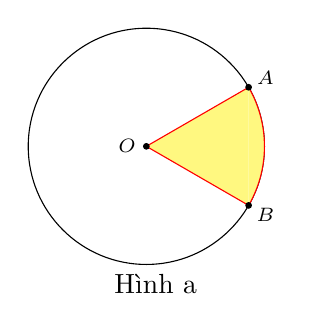
\begin{tikzpicture}[declare function={r=1.5;}]
	\path (0,0) coordinate (O);
	\foreach \goc/\bankinh/\t in {30/r/A,-30/r/B}{
	\path (\goc:\bankinh) coordinate (\t);
	}
	\draw (O) circle (r) ;
	\draw [red,fill=yellow!50](B) arc (-30:30:r);
	\draw [red,fill=yellow!50](A)--(O)--(B);
	\foreach \t/\g in {A/30,B/-30,O/180}{
	\draw[fill=black] (\t) circle (1pt) node[shift={(\g:7pt)},font=\scriptsize]{$ \t $};
	}
	\path (current bounding box.south) node[below, black]{Hình a};
	\end{tikzpicture}
	\hspace*{1cm}
	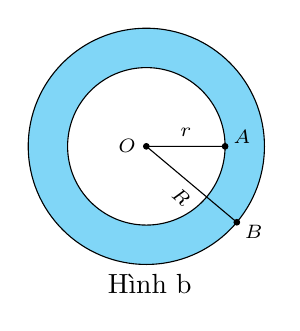
\begin{tikzpicture}[declare function={r=1;R=1.5;}]
	\path (0,0) coordinate (O);
	\foreach \goc/\bankinh/\t in {0/r/A,-40/R/B}{
	\path (\goc:\bankinh) coordinate (\t);
	}
	\draw [fill=cyan!50](O) circle (R);
	\draw [fill=white](O) circle (r);
	\draw (O)--(A) (O)--(B);
	\foreach \t/\g in {A/30,B/-30,O/180}{
	\draw[fill=black] (\t) circle (1pt) node[shift={(\g:7pt)},font=\scriptsize]{$ \t $};
	}
	\path (O)--(A)node[font=\scriptsize,midway, sloped, above]{$r$} (B)--(O)node[font=\scriptsize,midway, sloped, below]{$R$};
	\path (current bounding box.south) node[below, black]{Hình b};
	\end{tikzpicture}
	\hspace*{1cm}
	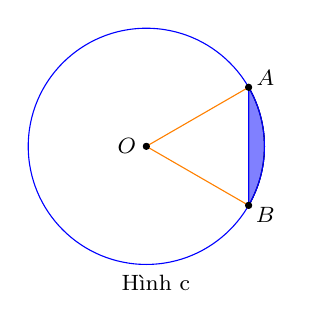
\begin{tikzpicture}[>=stealth,line join=round,line cap=round,font=\footnotesize,scale=1]
	\def\r{1.5} 
	\path 
	(0,0) coordinate (O)
	(30:\r) coordinate (A)
	(-30:\r) coordinate (B)
	;
	\draw[blue] (O) circle(\r);
	\draw[fill=blue!50] (B) arc(-30:30:\r)--(A)--(B);
	\draw[blue] (B) arc(-30:30:\r)--(A)--(B);
	\draw[orange] (A)--(O)--(B);
	\foreach \x/\y in {O/180,A/30,B/-30}
	\draw[fill=black] (\x) circle (1.1pt) + (\y:7pt) node{$\x$};
	\path (current bounding box.south) node[below, black]{Hình c};
	\end{tikzpicture}
\end{center}
\begin{boxdn}
	\begin{itemize}
	\item
	Hình quạt tròn là phần hình tròn giới hạn bởi một cung tròn và hai bán kính đi qua hai đầu mút của cung đó (Hình a).
	\item
	Hình vành khuyên (còn gọi là hình vành khăn) là phần nằm giữa hai đường tròn có cùng tâm và bán kính khác nhau (còn gọi là hai đường tròn đồng tâm) (Hình b).
	\item
	Hình viên phân là phần hình tròn được giới hạn bởi một cung và dây căng cung (Hình c).
	\end{itemize}
\end{boxdn}
\begin{boxdl}
	\begin{itemize}
	\item Diện tích $S_{\mathrm{q}}$ của hình quạt tròn bán kính $R$ ứng với cung $n^{\circ}$ là
	\begin{align}
	S_{q}=\dfrac{\pi R^2n}{360}=\dfrac{lR}{2}. \tag{3}
	\end{align}
	\item Diện tích $S_{\mathrm{v}}$ của hình vành khuyên tạo bởi hai đường tròn đồng tâm có bán kính $R$ và $r$.
	\begin{align}
	S_{v}=\pi\left(R^{2}-r^{2}\right)~(\text{với}~R>r). \tag{4}
	\end{align}
	\end{itemize}
\end{boxdl}
\begin{nx}
	Công thức (3) có thể viết là $S_{\mathrm{q}}=\dfrac{n}{360}S$ hay $\dfrac{S_{\mathrm{q}}}{S}=\dfrac{n}{360}=\dfrac{l}{C}$, nghĩa là
	tỉ số giữa diện tích hình quạt tròn ứng với cung $n^{\circ}$ và diện tích hình tròn (cùng bán kính) đúng bằng $\dfrac{n}{360}$ và bằng tỉ số giữa độ dài cung $n^{\circ}$ và độ dài đường tròn.
\end{nx}
\end{tomtat}
%%%%%%%%%%%%%%%%%%%%%
\subsection{Các dạng bài tập}
\begin{dang}{Tính độ dài đường tròn, cung tròn hoặc các đại lượng liên quan}
%	Dựa vào công thức $C = 2\pi $; $l = \dfrac{\pi Rn}{180}$; $R = \dfrac{C}{2\pi}$; $R = \dfrac{180l}{\pi n}$; $n = \dfrac{180 l}{\pi R}$
\end{dang}	
%%==========Ví dụ 1
\begin{vd}%[9H3B7]
	\begin{enumerate}
	\item Tính chu vi đường tròn biết đường kính là $5\, \mathrm{cm}$.
	\item Tính độ dài cung $120^{\circ}$ của đường tròn bán kính $4\, \mathrm{cm}$. 
	\end{enumerate}	
	\loigiai{
	\begin{enumerate}
	\item Chu vi đường tròn $C = 2\pi R = 5\pi\, \left(\mathrm{cm}\right)$.
	\item Độ dài cung $120^{\circ}$ của đường tròn bán kính $4\, \mathrm{cm}$ là $l = \dfrac{\pi R n}{180} = \dfrac{\pi\cdot 4\cdot 120}{180} = \dfrac{8\pi}{3}\, \left(\mathrm{cm}\right)$.
	\end{enumerate}	
	}
\end{vd}
%%==========Ví dụ 2
\begin{vd}
	Tính độ dài cung $40^{\circ}$ của đường tròn bán kính $9$ cm.
	\loigiai{
	Độ dài cung $40^{\circ}$ của đường tròn bán kính $9$ cm là
	$l=\dfrac{40}{180}\cdot\pi\cdot9=2\pi~\text{(cm)}.$
	}
\end{vd}
%%==========Ví dụ 3
\begin{vd}
	Tính độ dài cung $30^{\circ}$ của một đường tròn có bán kính $10 \mathrm{~cm}$.
	\loigiai{
	Cung $30^{\circ}$, bán kính $\mathrm{R}=10 \mathrm{~cm}$ có độ dài là: $l=\dfrac{\pi \mathrm{Rn}}{180}=\dfrac{\pi \cdot 10 \cdot 30}{180}=\dfrac{5 \pi}{3}$ $(\mathrm{cm})$.
	}
\end{vd}
%%==========Ví dụ 4
\begin{vd}
	Tính độ dài cung $72^{\circ}$ của một đường tròn có bán kính $25 \mathrm{~cm}$. (Lấy $\pi$ theo máy tính và làm tròn kết quả đến hàng phần trăm.)
	\loigiai{
	Cung $72^{\circ}$, bán kính $\mathrm{R}=25 \mathrm{~cm}$ có độ dài là: $l=\dfrac{\pi \mathrm{Rn}}{180}=\dfrac{\pi \cdot 25 \cdot 72}{180}=10 \pi \approx 31{,}4$ $(\mathrm{cm})$.
	}
\end{vd}
%%==========Ví dụ 5
\begin{vd}
	Cung có số đo $100^{\circ}$ của đường tròn bán kính $8$ cm dài bao nhiêu centimét (làm tròn kết quả đến hàng đơn vị)?
	\loigiai{
	Độ dài cung tròn đó là
	$
	\dfrac{100 \cdot \pi \cdot 8}{180}=\dfrac{40 \pi}{9} \approx 14$ (cm).
	}
\end{vd}
%%==========Ví dụ 6
\begin{vd}%[9H3B1]
	Cho đường tròn $\left(O;R\right)$ độ dài $\wideparen{AB}$ là $\dfrac{\pi R}{4}$. Tính $\text{sđ}\wideparen{AB}$.
	\loigiai{
	Gọi $n$ là số đo của cung nhỏ $\wideparen{AB}$. Ta có $l = \dfrac{\pi R n }{180}\Rightarrow \dfrac{\pi R}{4} = \dfrac{\pi R n }{180}\Rightarrow n = \dfrac{180}{4} = 45$. Do đó $\text{sđ}\wideparen{AB} = 45^{\circ}$.
	}
\end{vd}
%%==========Ví dụ 7
\begin{vd}
	Cho $A$ và $B$ là hai điểm trên đường tròn $(O;3\mathrm{~cm})$ sao cho $\widehat{AOB}=120^{\circ}$. Tính số đo và độ dài các cung có hai mút $A$, $B$.
	\loigiai{
	\immini{
	Ta có hai cung:
	\begin{itemize}
	\item Cung nhỏ $AB$ bị chắn bởi góc ở tâm $AOB$.\\
	Do đó sđ$\wideparen{AB}=\widehat{AOB}=120^{\circ}$;\\
	Độ dài $l_1$ của cung $AB$ là
	$
	l_1=\dfrac{120}{180} \cdot\pi \cdot 3=2 \pi~(\text{cm}).
	$
	\item Cung lớn $AmB$ có số đo là
	$
	\text{sđ}\wideparen{AmB}=360^{\circ}-120^{\circ}=240^{\circ} \text {.}
	$\\
	Độ dài $l_2$ của cung $AmB$ là
	$
	l_2=\dfrac{240}{180} \cdot\pi \cdot 3=4 \pi~(\text{cm}).
	$
	\end{itemize}
	}{
	\begin{tikzpicture}[declare function={r=1.5;}]
	\path (0,0) coordinate (O);
	\foreach \goc/\bankinh/\t in {30/r/A,150/r/B,-90/r/m}{
	\path (\goc:\bankinh) coordinate (\t);
	}
	\draw (O) circle (r) (A)--(O)--(B);
	\path(m)node[below] {$m$};
	\path pic["\scriptsize$120^\circ$", angle eccentricity=2,draw,angle radius=7pt]{angle= A--O--B};
	\foreach \t/\g in {A/30,B/150,O/-90}{
	\draw[fill=black] (\t) circle (1pt) node[shift={(\g:7pt)},font=\scriptsize]{$ \t $};
	}
	\end{tikzpicture}
	}
	}
\end{vd}
%%==========Ví dụ 8
\begin{vd}
	Một chất điểm chuyển động trên một đường tròn có bán kính $r=0{,}3$ m với tốc độ không đổi. Chất điểm chuyển động hết một vòng quanh đường tròn đó trong $20$ s. Tính tốc độ của chất điểm (theo đơn vị mét trên giây và làm tròn kết quả đến hàng phần trăm).
	\loigiai{
	Chu vi của đường tròn là $C=2 \pi \cdot 0,3=0,6 \pi$ (m).\\
	Vậy tốc độ của chất điểm là
	$v=\dfrac{0{,}6 \pi}{20} \approx 0{,}09$ (m/s).
	}
\end{vd}
%%==========Ví dụ 9
\begin{vd}
	\immini{Tính độ dài của đoạn hàng rào từ $A$ đến $B$ của sân cỏ trong hình bên, cho biết $\widehat{AOB}=80^{\circ}$.}{\begin{tikzpicture}
	\def\R{1.5}
	\path 
	(0:0) coordinate (O)
	+(-40:\R) coordinate (A)
	+(40:\R) coordinate (B);
	\draw (O) circle (\R);
	\draw (A)--(O);
	\draw (O)--(B) node[above, midway, sloped]{$10$ m};
	\draw pic[draw, angle radius = 10pt, "$80^\circ$", angle eccentricity = 2]{ angle = A--O--B};
	\foreach \x/\g in {O/180,A/-40,B/40}
	\fill (\x) circle (1.5pt)
	+(\g:3mm) node {$\x$};
	\end{tikzpicture}}
	\loigiai{
	Cung $80^{\circ}$, bán kính ${R}=10 $ m có độ dài là $l=\dfrac{\pi {Rn}}{180}=\dfrac{\pi \cdot 10 \cdot 80}{180}=8 \pi \approx 25{,}13$ $(\mathrm{m})$.
	}
\end{vd}
%%==========Ví dụ 10
\begin{vd}
	\immini{Một con lắc di chuyển từ vị trí $A$ đến vị trí $B$. Tính độ dài quãng đường $A B$ mà con lắc đó đã di chuyển, biết rằng sợi dây $O A$ có độ dài bằng $l$ và tia $O A$ tạo với phương thẳng đứng góc $\alpha$.}
	{\begin{tikzpicture}[>=stealth,line join=round,line cap=round,font=\footnotesize,scale=0.8]
	\def\r{3.5} 
	\path 
	(0,0) coordinate (O)
	(-120:\r) coordinate (A)
	(-60:\r) coordinate (B)
	(-90:\r) coordinate (C)
	($(C)!0.1!180:(O)$) coordinate (C')
	;
	\draw[dashed,blue] (A)--(O);
	\draw[blue] (O)--(B);
	\draw[dashed] (A) arc(-120:-60:\r);
	\draw[dashed,blue] (O)--(C');
	;
	\node at ($(O)+(-103:0.7)$){$\alpha$};
	\foreach \x/\y in {O/90,A/-190,B/-80}
	\draw[fill=black] (\x) circle (1.1pt) + (\y:0.5cm) node{$\x$};
	\draw pic[draw, angle radius=4mm, angle eccentricity=1.5]{angle = A--O--C};
	\draw pic[draw, angle radius=4.5mm, angle eccentricity=1.5]{ angle = C--O--B};
	\end{tikzpicture}}
	\loigiai{
	Góc được tạo thành khi con lắc di chuyển từ vị trí $A$ đến vị trí $B$ là $2\alpha$.\\
	Khi đó độ dài quãng đường con lắc đi được là $AB=\dfrac{\pi R\cdot 2\alpha}{180}=\dfrac{\pi R\cdot\alpha}{90}$ (đvđd).
	}
\end{vd}
%%==========Ví dụ 11
\begin{vd}
	\immini{
	Bánh xe (khi bơm căng) của một chiếc xe đạp có đường kính $650$ mm. Biết rằng khi giò đĩa quay một vòng thì bánh xe quay được khoảng $3{,}3$ vòng. Hỏi chiếc xe đạp di chuyển được quãng đường dài bao nhiêu mét sau khi người đi xe đạp $10$ vòng liên tục?\\
	\textit{Hướng dẫn:} Khi bánh xe quay $3{,}3$ vòng thì mỗi điểm trên bánh xe di chuyển được một độ dài bằnng $3{,}3$ lần chu vi đường tròn.
	}{
	\begin{tikzpicture}
	\tikzset{xedap/.pic={
	\shade[shading=radial] (-1.5,-2) rectangle (1.5,-1.6);
	\shade[shading=radial] (4.5,-2) rectangle (7.5,-1.6);
	\def\Radius{1.5cm}
	\foreach \a in {0, 10, ..., 350} {
	\draw[red] (0, 0) -- (\a:\Radius);
	\draw[black] (0, 0) -- (\a+1.5:\Radius);
	\draw[gray] (0, 0) -- (\a+3:\Radius);
	\draw[gray!50] (0, 0) -- (\a+4.5:\Radius);
	\draw[blue] (0, 0) circle[radius=\Radius];
	\draw[line width=4pt] (0, 0) circle[radius=\Radius+0.15cm];
	}
	\foreach \h in {0, 60, ..., 300} {
	\draw[color=black,line width=0.5mm,rotate around={\h:(0,0)}] (0,0) edge[-,bend left=40] (0.2cm,0) edge[-,bend right=40] (0.2cm,0);
	}
	\draw[line width=1pt] (0,0) circle[radius=0.2cm];
	\draw[line width=4pt,rounded corners=1pt,rotate=0] (1.68,0.6)--(1.94,0.54);
	\draw[line width=0.3mm,yellow!60!black] (1.8,0) arc (0:150:1.8cm)--(0,0);
	\draw[line width=0.5mm,yellow!60!black] (1.8,0) arc (0:160:1.8cm);
	\foreach \b in {0, 10, ..., 350} {
	\draw[color=red,rotate around={\b:(6,0)}] (6, 0) -- (7.5,0);
	\draw[black,rotate around={\b+1.5:(6,0)}] (6, 0) -- (7.5,0);
	\draw[gray,rotate around={\b+3:(6,0)}] (6, 0) -- (7.5,0);
	\draw[gray!50,rotate around={\b+4.5:(6,0)}] (6, 0) -- (7.5,0);
	\draw[blue] (6, 0) circle[radius=\Radius];
	\draw[line width=4pt] (6, 0) circle[radius=\Radius+0.15cm];
	}
	\draw[line width=0.3mm,yellow!60!black] (6,1.8) arc (90:190:1.8cm)--(6,0);
	\draw[line width=0.5mm,yellow!60!black] (6,1.8) arc (90:200:1.8cm);
	\draw[line width=1pt] (0,0.2cm)--(2.2,0.5cm) (0,-0.2cm)--(2.2,-0.5cm);
	\draw[line width=2pt] (2.2,0)--(2.6,-0.6) (2.2,0)--(1.8,0.6);
	\draw[line width=1mm,rounded corners=8pt,rotate around={25:(6,0)}] (6,0)--(6,1.3cm)--++(80:2.1cm);
	\draw[line width=1mm,rounded corners=8pt,rotate around={27:(6,0)}] (6,0)--(6,1.3cm)--++(80:2.1cm);
	\draw[line width=1mm,rounded corners=8pt,rotate around={26:(6,0)}] (6,0)--(6,1.3cm)--++(80:2.1cm)coordinate(a);
	\draw[line width=1.5mm] (a)--++(-80:0.15cm)--++(0:0.5cm)--++(180:0.05cm)coordinate(b);
	\draw[line width=1.1mm,rounded corners=4pt] (b)--++(-30:0.6cm)coordinate(c)--++(-160:0.4cm) (b)--++(150:0.6cm)coordinate(d)--++(200:0.4cm);
	\draw[line width=0.4mm,rounded corners=0pt] (c)--++(-95:0.1cm)--++(-160:0.25cm) (d)--++(-95:0.1cm)--++(200:0.25cm);
	\draw[line width=2mm,rotate around={35:(2.2,0)}] (2.2,0)--++(3.7,0)--++(75:0.4cm)--++(155:3.5)coordinate(e)--(2.2,0);
	\draw[line width=1mm] (0,0)--(2.2,0) (0,0)--(45:2.5cm) (0,0)--(46.5:2.5) (0,0)--(2:2.2);
	\draw[line width=1.2mm] (e)--++(106:0.9cm)--++(-74:0.1cm)coordinate(d);
	\foreach \c in {0, 72, ..., 288} {\draw[color=red,line width=1.8mm,rotate around={\c:(2.2,0)}] (2.2,0) edge[-,bend left=30] (2.69,0);}
	\draw[line width=2pt] (2.2,0) circle[radius=0.5cm];
	\fill (2.2,0) circle[radius=0.1cm];
	\draw[line width=4pt,rounded corners=1pt,rotate=0] (2.4,-0.58)--(2.68,-0.56);
	\draw[line width=2pt] (2.2,0)--(2.6,-0.6);
	\shade[top color=white,bottom color=black,rounded corners=2pt,rotate around={10:(d)}] (d)--++(220:2mm)--++(100:2mm)--++(180:3mm)--++(110:1.5mm)--++(160:2mm)--++(110:3.5mm)coordinate(i)--++(-15:10mm)--++(-5:5mm)--++(-20:3mm)coordinate(j)--++(-50:0.7mm)--++(180:4mm)--++(170:1mm)--++(-175:2mm)--(d);
	\shade[top color=gray!50,bottom color=black,rounded corners=2pt,rotate around={10:(d)}] (d)--++(220:2mm)--++(100:2mm)--++(180:3mm)--++(110:1.5mm)--++(160:2mm)--++(110:3.5mm)--++(-50:4.5mm)--++(-3:13mm)--++(-10:2mm)--++(180:4mm)--++(170:1mm)--++(-175:2mm)--(d);
	\filldraw[black] (0,0)circle(2pt) (6,0)circle(2pt);
	\draw[line width=0.3mm] (0,0)--++(105:2cm)--++(-2:0.7cm)coordinate(g)--+(-10:1.5cm) (g)--(0,0);
	\shade[top color=gray!10!white,bottom color=gray] (-0.8cm,1.9cm)--++(-3:1.4cm) arc (-90:90: 0.4mm)--++(174:1.4cm) arc (90:270: 0.65mm);
	\shade[top color=gray!20,bottom color=black] (-0.8cm,1.9cm)--++(-3:1.4cm) arc (-90:90: 0.4mm)--++(177:1.4cm) arc (90:270: 0.4mm);	
	}}
	\path (0,0) pic[rotate=0,scale=0.75]{xedap};
	\draw [<-,thick](1.7,-0.45)--(2,-1.2) node[below,font=\scriptsize]{Giò đĩa};
	\end{tikzpicture}
	}
	\loigiai{
	Chu vi của bánh xe là \[C=\pi\cdot650=650\pi~\text{(mm).}\]
	Khi đạp giò đĩa $10$ vòng thì bánh xe quay được \[10\cdot3{,}3=33~\text{(vòng)}.\]
	Khi đó mỗi điểm trên bánh xe di chuyển được quãng đường là \[l=33\cdot650\pi\approx33\cdot650\cdot3{,}14=67353~\text{(mm)}=67{,}353~\text{(m)}.\]
	Vậy người đi xe đạp giò đĩa $10$ vòng liên tục thì xe đạp di chuyển được quãng đường xấp xỉ $67{,}353$ m.
	}
\end{vd}	
%%==========Ví dụ 12
\begin{vd}%[9H3K7]
	Cho nửa đường tròn đường kính $AB$. Trong đoạn thẳng $AB$ lấy hai điểm $M$, $N$ ($M$ nằm giữa $A$ và $N$). Vẽ các nửa đường tròn đường kính $AM$, $MN$, $NB$. Chứng minh tổng độ dài của ba đường tròn đường kính $AM$, $MN$, $NB$ bằng độ dài nửa đường tròn đường kính $AB$.
	\loigiai{
	\immini
	{Gọi $C_{1}$, $C_{2}$, $C_{3}$, $C$ lần lượt là độ dài của nửa đường tròn đường kính $AM$, $MN$, $NB$, $AB$.\\
	Ta có $C_{1} = \dfrac{1}{2}\cdot\pi\cdot AM$, $C_{2} = \dfrac{1}{2}\cdot\pi\cdot MN$, $C_{3} = \dfrac{1}{2}\cdot\pi\cdot NB$ và $C = \dfrac{1}{2}\cdot\pi\cdot AB$.\\
	Khi đó 
	\allowdisplaybreaks
	\begin{eqnarray*}
	C_{1} + C_{2} + C_{3} &=& \dfrac{1}{2}\cdot\pi\cdot AM + \dfrac{1}{2}\cdot\pi\cdot MN + \dfrac{1}{2}\cdot\pi\cdot NB\\
	&=& \dfrac{1}{2}\cdot\pi\left(AM + MN + NB\right) = \dfrac{1}{2}\cdot\pi\cdot AB.
	\end{eqnarray*}
	Do đó $C_{1} + C_{2} + C_{3} = C$.
	}
	{\begin{tikzpicture}[line join = round, line cap = round,>=stealth,scale=1]
	\tkzDefPoints{0/0/A}
	\tkzDefShiftPoint[A](0:6){B}
	\tkzDefMidPoint(A,B)\tkzGetPoint{O}
	\coordinate (M) at ($(A)!0.4!(B)$);
	\coordinate (N) at ($(A)!0.75!(B)$);
	\tkzDefMidPoint(A,M)\tkzGetPoint{I}
	\tkzDefMidPoint(N,M)\tkzGetPoint{J}
	\tkzDefMidPoint(N,B)\tkzGetPoint{K}
	\pgfresetboundingbox
	\tkzDrawSegments(A,B)
	\tkzDrawPoints[fill=black](A,B,O,M,N,I,J,K)
	\tkzLabelPoints[below](A,B,M,N)
	\tkzDrawArc[rotate,color = black, line width = 0.6pt](O,B)(180)
	\tkzDrawArc[rotate,color = black, line width = 0.6pt](I,M)(180)
	\tkzDrawArc[rotate,color = black, line width = 0.6pt](J,N)(180)
	\tkzDrawArc[rotate,color = black, line width = 0.6pt](K,B)(180)
	\end{tikzpicture}
	}	
	}
\end{vd}
%===================
\begin{dang}{Tính diện tích hình tròn, hình quạt tròn và những yếu tố liên quan}
\end{dang}
%%==========Ví dụ 13
\begin{vd}%[9H3B10]
	\begin{enumerate}
	\item Tính diện tích hình tròn bán kính $5$ cm.
	\item Tính diện tích hình quạt tròn bán kính $6$ cm có số đo cung là $60^\circ$.
	\end{enumerate}
	\loigiai
	{ 	
	\begin{enumerate}
	\item Diện tích hình tròn bán kính $5$ cm là: $S=\pi R^2 = 25 \pi$ (cm$^2$).
	\item Diện tích hình quạt tròn là: $S_\text{q} = \dfrac{\pi R^2n}{360}=\dfrac{\pi\cdot 6^2 \cdot 60}{360}=6\pi$ (cm$^2$).
	\end{enumerate}
	}
\end{vd}
%%==========Ví dụ 14
\begin{vd}
	\immini{Bề mặt phía trên của một chiếc trống có dạng hình tròn bán kính $8 \mathrm{~cm}$. Diện tích bề mặt phía trên của trống đó bằng bao nhiêu centimét vuông (làm tròn kết quả đến hàng đơn vị)?}
	{
\includegraphics[scale=0.8]{images/images-9C5-5/Hinh70-Vidu3-C5-Bai5-Dodaicungtron.png}}	
	\loigiai{
	Diện tích bề mặt phía trên của chiếc trống đó là
	$
	S=\pi \cdot 8^2=64 \pi \approx 201$ (cm$^2$).
	}
\end{vd}
%%==========Ví dụ 15
\begin{vd}
	Tính diện tích của hình quạt tròn bán kính $5$ cm và có độ dài cung tương ứng với nó bằng $4\pi$ cm.
	\loigiai{
	Theo đề bài, hình quạt tròn có độ dài cung tương ứng với nó là $l=4\pi$ cm, bán kính là $R=5$ cm.\\
	Do đó, diện tích $S$ của nó là\\
	\[
	S=\dfrac{l\cdot R}{2}=\dfrac{4\pi\cdot5}{2}=10 \pi\left(\text{cm}^{2}\right).
	\]
	}
\end{vd}
%%==========Ví dụ 16
\begin{vd}
	Tính diện tích hình quạt tròn bán kính $\mathrm{R}=10 \mathrm{~cm}$, ứng với cung $60^{\circ}$ (kết quả làm tròn đến hàng phần trăm của $\mathrm{cm}^2$).
	\loigiai{
	Hình quạt tròn bán kính $\mathrm{R}=10 \mathrm{~cm}$, ứng với cung $60^{\circ}$ có diện tích là
	\[
	S=\dfrac{\pi \mathrm{R}^2 \mathrm{n}}{360}=\dfrac{\pi \cdot 10^2 \cdot 60}{360} \approx 52{,}36\ \left(\mathrm{cm}^2\right) .
	\]
	}
\end{vd}
%%==========Ví dụ 17
\begin{vd}
	Tính diện tích hình quạt tròn bán kính $\mathrm{R}=20 \mathrm{~cm}$, ứng với cung $72^{\circ}$.
	\loigiai{
	Diện tích hình quạt tròn là
	\[
	S=\dfrac{\pi \mathrm{R}^2 \cdot 72}{360}=\dfrac{\pi \cdot 20 \cdot 72}{360}=4\pi \approx 12{,}57\ \left(\mathrm{cm}^2\right).
	\]
	}
\end{vd}
%%==========Ví dụ 18
\begin{vd}
	\immini
	{Tính diện tích của miếng bánh pizza có dạng hình quạt tròn trong hình bên. Biết $OA=15 \mathrm{~cm}$ và $\widehat{AOB}=55^{\circ}$.}
	{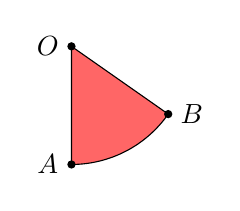
\begin{tikzpicture}
	\def\R{1.5}
	\path 
	(0:0) coordinate (O)
	+(-90:\R) coordinate (A)
	+(-35:\R) coordinate (B);
	\fill[red!60!white] (O)--(A) arc (-90:-35:\R)--(B)--cycle;
	\draw (A)--(O)--(B);
	\draw (0,-\R) arc (-90:-35:\R);
	\foreach \x/\g in {O/180,A/180,B/0}
	\fill (\x) circle (1.5pt)
	+(\g:3mm) node {$\x$};
	\end{tikzpicture}}
	\loigiai{
	Diện tích của miếng bánh pizza là
	\[
	S=\dfrac{\pi \mathrm{OA}^2 \cdot\widehat{AOB} }{360}=\dfrac{\pi \cdot 15 \cdot 55}{360} \approx 7{,}2\ \left(\mathrm{cm}^2\right).
	\]
	}
\end{vd}
%%==========Ví dụ 19
\begin{vd}
	\immini{Cho hình quạt tròn $A O B$ giới hạn bởi hai bán kính $O A$, $O B$ và cung $A m B$ sao cho $O A=A B$. Hãy tìm số đo cung $A m B$ ứng với hình quạt đó.}
	{\begin{tikzpicture}[>=stealth,line join=round,line cap=round,font=\footnotesize,scale=1]
	\def\r{1.5} 
	\path 
	(0,0) coordinate (O)
	(0:\r) coordinate (B)
	(60:\r) coordinate (A)
	;
	\draw[blue] (O) circle(\r);
	\draw[fill=orange!50] (O)--(B) arc(0:60:\r)--(A)--(O)--cycle;
	\draw[orange] (O)--(B) arc(0:60:\r)--(A)--(O)--cycle (A)--(B);
	%	;
	%	\draw[orange] (O)--(N);
	\node at ($(O)+(20:\r+0.3)$){$m$};
	\foreach \x/\y in {O/-100,A/90,B/0}
	\draw[fill=black] (\x) circle (1.1pt) + (\y:0.3cm) node{$\x$};
	\end{tikzpicture}}
	\loigiai{
	Do $O A=A B$ nên tam giác $A O B$ là tam giác đều, suy ra $\widehat{A O B}=60^{\circ}$.\\ Vì góc $A O B$ là góc ở tâm chắn cung $A m B$ nên $\text{sđ}\wideparen{A O B}=60^{\circ}$.
	}
\end{vd}
%%==========Ví dụ 20
\begin{vd}
	\immini{Cho hình quạt tròn $C O D$ giới hạn bởi hai bán kính $O C$, $O D$ và cung $C m D$ sao cho $O C=C D$. Hãy tìm số đo cung $C m D$ ứng với hình quạt đó.}
	{\begin{tikzpicture}[>=stealth,line join=round,line cap=round,font=\footnotesize,scale=1]
	\def\r{1.5} 
	\path 
	(0,0) coordinate (O)
	(0:\r) coordinate (D)
	(60:\r) coordinate (C)
	;
	\draw[fill=orange!50] (O)--(C) arc(60:360:\r)--(D)--(O)--cycle;
	\draw[orange] (O)--(D) arc(0:60:\r)--(C)--(O)--cycle (C)--(D);
	\draw[blue] (O) circle(\r);
	\node at ($(O)+(-170:\r+0.3)$){$m$};
	\foreach \x/\y in {O/-100,C/90,D/0}
	\draw[fill=black] (\x) circle (1.1pt) + (\y:0.3cm) node{$\x$};
	\end{tikzpicture}}
	\loigiai{
	Do $O C=CDB$ nên tam giác $C O D$ là tam giác đều, suy ra $\widehat{C O D}=60^{\circ}$.\\
	Vì góc $C O D$ là góc ở tâm chắn cung $C n D$ nên $\text{sđ}\widehat{C O D}=60^{\circ}$.\\
	Do đó $\text{sđ} \widehat{CmD}=360^{\circ}-60^{\circ}=300^{\circ}$.
	}
\end{vd}
%%==========Ví dụ 21
\begin{vd}
	\immini{Một hoạ tiết trang trí có dạng hình tròn bán kính $4$ dm được chia thành nhiều hình quạt tròn, mỗi hình quạt tròn có góc ở tâm là $7{,}5^{\circ}$. Diện tích của mỗi hình quạt đó là bao nhiêu dm$^2$ (làm tròn kết quả đến hàng phần trăm)?}
	{
\includegraphics[scale=0.7]{images/images-9C5-5/hinh76-Vd5-C5-Bai5-Dodaicungtron.png}}
	\loigiai{
	Diện tích của mỗi hình quạt là $\dfrac{\pi \cdot 4^2 \cdot 7{,}5}{360} \approx 1{,}05 $ (dm$^2$).
	}
\end{vd}
%%==========Ví dụ 22
\begin{vd}
	\immini{Hình quạt ở hình bên có bán kính bằng $2$ dm và góc ở tâm bằng $150^{\circ}$.
	\begin{enumerate}
	\item Tính diện tích của hình quạt đó theo đơn vị decimét vuông (làm tròn kết quả đến hàng phẩn trăm).
	\item Tính chiều dài cung tương ứng với hình quạt tròn đó.
	\end{enumerate}}
	{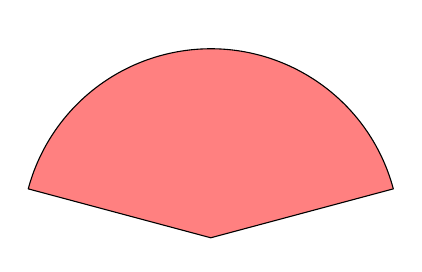
\begin{tikzpicture}[>=stealth,line join=round,line cap=round,font=\footnotesize,scale=0.8]
	\def\ra{3}
	\def\rb{0.4} 
	\path 
	(0,0) coordinate (O)
	(15:\ra) coordinate (B)
	(165:\ra) coordinate (A)
	(-15:\rb) coordinate (B')
	(-165:\rb) coordinate (A')
	;
	\draw[fill=red!50] (O)--(B) arc(15:165:\ra)--(A)--(O);
%	\draw[fill=orange!50] (O)--(B') arc(-15:-165:\rb)--(A')--(O);
	\end{tikzpicture}}
	\loigiai{
	\begin{enumerate}
	\item Diện tích của hình quạt là $\dfrac{\pi\cdot 2^2\cdot 150}{360}\approx 5{,}24 $ (dm$^2$).
	\item Ta có $S=\dfrac{lR}{2}$ nên chiều dài cung tương ứng với hình quạt tròn là $l=\dfrac{2S}{R}=\dfrac{2\cdot 5{,}24}{2}\approx 5{,}24$ (dm).
	\end{enumerate}	
	}
\end{vd}
%===================
\begin{dang}{Tính diện tích hình vành khăn, hình viên phân và những yếu tố liên quan}
\end{dang}
%%==========Ví dụ 23
\begin{vd}
	Tính diện tích của hình vành khuyên nằm giữa hai đường tròn đồng tâm có bán kính là $3$m và $5$m.
	\loigiai{
	Diện tích hình vành khuyên nằm giữa hai đường tròn đồng tâm có bán kính là $3$m và $5$m là
	$$S=\pi\left(\mathrm{R}^2-\mathrm{r}^2\right)=\pi\left(5^{2}-3^{2}\right)=16 \pi \, \mathrm{(m^2)}.$$
	}
\end{vd}
%%==========Ví dụ 24
\begin{vd}
	Tính diện tích của hình vành khuyên, biết hình vành khuyên đó giới hạn bởi hai đường tròn cùng tâm và có bán kính lần lượt là $2{,}5$ cm; $2$ cm.
	\loigiai{
	Tính diện tích của hình vành khuyên nằm giữa hai đường tròn đồng tâm có bán kính là $2{,}5$ cm và $2$ cm là
	$$S=\pi\left(\mathrm{R}^2-\mathrm{r}^2\right)=\pi\left(2{,}5^2-2^2\right)=\dfrac{9\pi}{4} \approx 7{,}07\,\mathrm{(cm^2)}.$$
	}
\end{vd}
%%==========Ví dụ 25
\begin{vd}
	Tính diện tích hình vành khuyên giới hạn bởi hai đường tròn $(O;5 \mathrm{~cm})$ và $(O;8 \mathrm{~cm})$ (kết quả làm tròn đến hàng phần trăm).
	\loigiai{
	Diện tích hình vành khuyên giới hạn bởi hai đường tròn $(O;5 \mathrm{~cm})$ và $(O;8 \mathrm{~cm})$ là \[S=\pi\left(\mathrm{R}^2-\mathrm{r}^2\right)=\pi\left(8^2-5^2\right)=39 \pi \approx 122{,}52\ \left(\mathrm{cm}^2\right).\]
	}
\end{vd}
%%==========Ví dụ 26
\begin{vd}
	Tính diện tích hình vành khuyên giới hạn bởi hai đường tròn $(O;10 \mathrm{~cm})$ và $(O;20 \mathrm{~cm})$ (kết quả làm tròn đến hàng phần trăm).
	\loigiai{
	Diện tích hình vành khuyên giới hạn bởi hai đường tròn $(O;10 \mathrm{~cm})$ và $(O;20 \mathrm{~cm})$ là \[S=\pi\left(\mathrm{R}^2-\mathrm{r}^2\right)=\pi\left(20^2-10^2\right)=300 \pi \approx 942{,}48\ \left(\mathrm{cm}^2\right).\]}
\end{vd}
%%==========Ví dụ 27
\begin{vd}
	\immini{Hình bên mô tả mặt cắt của một khúc gỗ có dạng một phần tư hình vành khuyên, trong đó hình vành khuyên giới hạn bởi hai đường tròn cùng tâm và có bán kính lần lượt là $4$ dm và $3$ dm. Diện tích mặt cắt đó là bao nhiêu decimét vuông (làm tròn kết quả đến hàng phần mười)?}
	{\begin{tikzpicture}[>=stealth,line join=round,line cap=round,font=\footnotesize,scale=0.8]
	\def\rn{3}
	\def \rl{3.6}
	\path 
	(0,0) coordinate (O)
	(-90:\rn) coordinate (M)
	(-90:\rl) coordinate (N)
	(M) arc (-90:0:\rn)coordinate (M')
	(N) arc (-90:0:\rl)coordinate (N')
	;
	\draw[dashed] (O)--(M) (O)--(M');
	\draw[fill=orange!50] (M)--(N)arc (-90:0:\rl)--(N')--(M') arc(0:-90:\rn)--cycle;
	\draw[green] (M)--(N)arc (-90:0:\rl)--(N')--(M') arc(0:-90:\rn)--cycle;
	\draw pic[draw, angle radius=2mm, angle eccentricity=1.5]{right angle = M--O--M'};
	\end{tikzpicture}}
	\loigiai{
	Diện tích của mặt cắt là $ \dfrac{1}{4} \pi\left(4^2-3^2\right)=\dfrac{7 \pi}{4} \approx 5{,}5$ (dm$^2$).
	}
\end{vd}
%%==========Ví dụ 28
\begin{vd}
	\immini{
	Một tấm bia tạo bởi năm đường tròn đồng tâm lần lượt có bán kính là $5$ cm, $10$ cm, $15$ cm, $20$ cm và $30$ cm. Giả thiết rằng người chơi ném phi tiêu một cách ngẫu nhiên và luôn trúng bia. Tính xác suất ném trúng vòng 8 (hình vành khuyên nằm giữa đường tròn thứ hai và thứ ba), biết rằng xác suất cần tìm bằng tỉ số giữa diện tích của hình vành khuyên tương ứng với diện tích của hình tròn lớn nhất.
	}{
	\begin{tikzpicture}[declare function={r1=0.5;r2=1;r3=1.5;r4=2;r5=3;},scale=0.65]
	\path (0,0) coordinate (O);
	\foreach \goc/\bankinh/\t in {-135/r1/A,-135/r2/B,-135/r3/C,-135/r4/D}{
	\path (\goc:\bankinh) coordinate (\t);
	}
	\draw [fill=cyan!20](O) circle (r5);
	\draw (O) circle (r1);
	\draw (O) circle (r2);
	\draw (O) circle (r3);
	\draw (O) circle (r4);
	\fill[red] (O) circle (2pt);
	\foreach \x/\y/\noidung in {A/-135/9,B/-135/8,C/-135/7,D/-135/6}{\fill[white] ($(\x)+(\y:0.25cm)$)node[red]{$\noidung$};}
	\end{tikzpicture}
	}
	\loigiai{
	Diện tích hình vành khuyên nằm giữa đường tròn thứ hai và thứ ba là
	\[S_{8}=\pi\left(15^2-10^2\right)=125\pi~\left(\text{cm}^2\right).\] 
	Diện tích hình tròn lớn nhất
	\[S=\pi\cdot30^2=900\pi~\left(\text{cm}^2\right).\]
	Xác suất ném trúng vòng $8$ là
	\[\dfrac{125\pi}{900\pi}=\dfrac{5}{36}.\]
	}
\end{vd}
%%==========Ví dụ 29
\begin{vd}
	\immini
	{Cho hình vành khuyên giới hạn bởi hai đường tròn $(O;\mathrm{r})$ và $(O;\mathrm{R})$ với $\mathrm{R}>\mathrm{r}$. Trên đường tròn $(O;\mathrm{R})$ lấy hai điểm $B$, $C$ sao cho $BC$ vừa là dây cung của $(O;\mathrm{R})$, vừa vuông góc với bán kính của đường tròn $(O;\mathrm{r})$ tại $A$ (hình bên).
	\begin{enumerate}
	\item Tính độ dài đoạn thẳng $BC$ theo $\mathrm{r}$ và $\mathrm{R}$.
	\item Cho $BC=a \sqrt{3}$. Tính diện tích hình vành khuyên giới hạn bởi hai đường tròn $(O; \mathrm{r})$ và $(O; \mathrm{R})$ theo $a$.
	\end{enumerate}}
	{\begin{tikzpicture}[scale=0.85]
	\def \R{2}
	\def \r{1.3333333}
	\path 
	(0:0) coordinate (O)
	+(-41.81:\R) coordinate (B)
	+(-138.19:\R) coordinate (C)
	+(-90:\r) coordinate (A);
	\draw[fill=green!30!white] (O) circle (\R);
	\draw[fill = white] (O) circle (\r);
	\fill (A) circle (1.5pt) (B) circle (1.5pt);
	\draw pic[draw, angle radius = 6pt]{right angle = B--A--O};
	\draw 
	(C)--(B)
	(O)--(B) node[above,midway,sloped]{$R$}
	(A)--(O) node[above,midway,sloped]{$r$};
	\foreach \x/\g in {O/100,A/-90,B/-40,C/-140}
	\fill (\x) circle (1.5pt)
	+(\g:3mm) node {$\x$};
	\end{tikzpicture}}
	\loigiai{
	\begin{enumerate}
	\item $BC=2AB=2\sqrt{OB^2-OA^2}=2\sqrt{\mathrm{R}^2-\mathrm{r}^2}.$.
	\item Diện tích hình vành khuyên giới hạn bởi hai đường tròn $(O; \mathrm{r})$ và $(O; \mathrm{R})$ là
	\[S=\pi\left(\mathrm{R}^2-\mathrm{r}^2\right)=\pi\left(\dfrac{BC}{2}\right)^2=\pi\left(\dfrac{a \sqrt{3}}{2}\right)^2=\dfrac{3\pi}{4}a^2\ \left(\mathrm{cm}^2\right).\]
	\end{enumerate}
	}
\end{vd}
%%==========Ví dụ 30
\begin{vd}
	\immini
	{Phần hình tròn được giới hạn bởi một cung và dây căng cung đó gọi là \textit{hình viên phân}. Tính diện tích hình viên phân $AmB$, biết góc ở tâm $\widehat{AOB}=60^{\circ}$ và bán kính đường tròn là $5{,}1 \mathrm{~cm}$ (hình bên) (kết quả làm tròn đến hàng phần trăm của $\mathrm{cm}^2$).}
	{\begin{tikzpicture}
	\def\R{1.5}
	\path 
	(0:0) coordinate (O)
	+(-100:\R) coordinate (A)
	+(-70:\R) coordinate (M) node [below] {m}
	+(-40:\R) coordinate (B);
	\draw (O) circle (\R);
	\fill[pattern = north east lines] (O)--(A) arc (-100:-40:\R)--(B)--cycle;
	\draw[fill=white] (A)--(B)--(O)--cycle;
	\draw pic[draw, angle radius = 10pt, "$60^\circ$", angle eccentricity = 2]{ angle = A--O--B};
	\foreach \x/\g in {O/180,A/-100,B/-40}
	\fill (\x) circle (1.5pt)
	+(\g:3mm) node {$\x$};
	\end{tikzpicture}}
	\loigiai{
	Ta có $OAB$ là tam giác đều cạnh $\mathrm{R}$, suy ra
	\[
	S_{OAB}=\dfrac{\mathrm{R}^2 \sqrt{3}}{4}=\dfrac{5{,}1^2 \cdot \sqrt{3}}{4} \approx 11{,}26\ \left(\mathrm{cm}^2\right).
	\]
	Diện tích hình quạt tròn $OAmB$ là
	\[
	S_{OAmB}=\dfrac{\pi \mathrm{R}^2 \cdot 60}{360}=\dfrac{\pi \cdot 5{,}1^2 \cdot 60}{360} \approx 13{,}62\ \left(\mathrm{cm}^2\right).
	\]
	Suy ra diện tích hình viên phân $AmB$ là
	\[
	S_{AmB}=S_{OAMB}-S_{OAB} \approx 13{,}62-11{,}26=2{,}36\ \left(\mathrm{cm}^2\right).
	\]
	}
\end{vd}
%%==========Ví dụ 31
\begin{vd}
	Hình viên phân là hình giới hạn bởi một cung tròn và dây cung (tương ứng) của đường tròn (minh hoạ bởi phần tô đậm ở Hình a).
	Người ta làm một hoạ tiết trang trí bằng cách ghép hai hình viên phân bằng nhau (Hình b), mỗi hình viên phân đó có góc ở tâm tương ứng là $90^{\circ}$ và bán kính đường tròn tương ứng là $2$ dm (Hình c). Tính diện tích của hoạ tiết trang trí đó (theo đơn vị decimét vuông và làm tròn kết quả đến hàng phần trăm).
	\begin{center}
	\begin{tabular}{ccc}
	\begin{tikzpicture}[>=stealth,line join=round,line cap=round,font=\footnotesize,scale=0.8]
	\def\r{2} 
	\path 
	(0,0) coordinate (O)
	(45:\r) coordinate (A)
	(-45:\r) coordinate (B)
	;
	\draw[blue] (O) circle(2);
	\draw[fill=blue!50] (B) arc(-45:45:\r)--(A)--(B);
	\draw[blue] (B) arc(-45:45:\r)--(A)--(B);
	\draw[orange] (A)--(O)--(B);
	\foreach \x/\y in {O/180,A/90,B/-90}
	\draw[fill=black] (\x) circle (1.1pt) + (\y:0.5cm) node{$\x$};
	\draw (0,-2.5)node[below]{$\text{Hình a}$ } ;
	\end{tikzpicture}
	&
	\begin{tikzpicture}[>=stealth,line join=round,line cap=round,font=\footnotesize,scale=0.8]
	\def\r{2} 
	\path 
	(0,0) coordinate (O)
	(45:\r) coordinate (A)
	(-45:\r) coordinate (B)
	($(A)!(O)!(B)$) coordinate (H)
	($(H)!1!180:(O)$) coordinate (O')
	;
	\draw[fill=orange!50] (B) arc(-45:45:\r)--(A)--(B);
	\draw[fill=orange!50] (A) arc(135:225:\r)--(B)--(A);
	\draw[orange] (B) arc(-45:45:\r)--(A)--(B) (A) arc(135:225:\r)--(B)--(A);
	\draw (1.3,-2.5)node[below]{$\text{Hình b}$ } ;
	\end{tikzpicture}
	& \begin{tikzpicture}[>=stealth,line join=round,line cap=round,font=\footnotesize,scale=0.8]
	\def\r{2} 
	\path 
	(0,0) coordinate (O)
	(45:\r) coordinate (B)
	(135:\r) coordinate (A)
	;
	%\draw[blue] (O) circle(2);
	\draw[fill=orange!50] (B) arc(45:135:\r)--(A)--(B);
	\draw[orange](B) arc(45:135:\r)--(A)--(O);
	\draw[orange] (O)--(B)node[pos=0.5,right]{$2$ dm};
	\foreach \x/\y in {O/-90,A/180,B/0}
	\draw[fill=black] (\x) circle (1.1pt) + (\y:0.5cm) node{$\x$};
	\draw (0,-0.9)node[below]{$\text{Hình c}$ } ;
	\end{tikzpicture}
	\end{tabular}
	\end{center}
	\loigiai{
	Trong Hình $79$, ta có
	\begin{itemize}
	\item Diện tích tam giác $O A B$ là
	$
	S_1=\dfrac{1}{2} O A \cdot O B=\dfrac{1}{2} \cdot 2 \cdot 2=2$ (dm$^2$);
	\item Do $\text{sđ}\wideparen{A B}=90^{\circ}$ nên diện tích hình quạt tròn $A O B$ tương ứng là\\
	$S_2=\dfrac{\pi \cdot 2^2 \cdot 90}{360}=\pi$ (dm$^2$).
	\end{itemize}
	Suy ra diện tích hình viên phân là $S_3=S_2-S_1=\pi-2$ (dm$^2$).\\
	Vậy diện tích của hoạ tiết trang trí đó là $S=2 S_3=2(\pi-2) \approx 2{,}28$ (dm$^2$).
	}
\end{vd}
%%==========Ví dụ 32
\begin{vd}%[9H3B10]
	Cho lục giác đều $ABCDEF$ nội tiếp đường tròn ($O$; $2$ cm). Tính diện tích phần hình tròn nằm bên ngoài hình lục giác.
	\loigiai
	{
	\immini{Số đo cung $AB$ là: $\dfrac{360^\circ}{6}=60^\circ$.\\
	Diện tích hình quạt $OAB$ là
	$$S_\text{q} = \frac{\pi R^2 n}{360}=\frac{\pi \cdot 2^2 \cdot 60}{360}=\frac{2\pi}{3}.$$
	$\triangle AOB$ có $OA=OB$, $\widehat{AOB}=60^\circ$ nên $\triangle AOB$ đều, do đó $AB=OA=OB=R.$ \\
	Vẽ $AH \perp AB,$ ta có: $OH=HB=\dfrac{R}{2}.$\\}
	{\begin{tikzpicture}[line join = round, line cap = round,>=stealth,scale=1]
	\tkzDefPoints{0/0/O}
	\tkzDefShiftPoint[O](90:2){A}
	\tkzDefPointBy[rotation = center O angle -60](A) \tkzGetPoint{B}
	\tkzDefPointBy[rotation = center O angle -60](B) \tkzGetPoint{C}
	\tkzDefPointBy[rotation = center O angle -60](C) \tkzGetPoint{D}
	\tkzDefPointBy[rotation = center O angle -60](D) \tkzGetPoint{E}
	\tkzDefPointBy[rotation = center O angle -60](E) \tkzGetPoint{F}
	\tkzDefPointBy[projection=onto B--O](A)\tkzGetPoint{H}
	\pgfresetboundingbox
	\tkzDrawSegments(O,A A,B B,C C,D D,E E,F O,B A,H F,A)
	\tkzDrawPoints[fill=black](A,B,O,C,D,E,F,H)
	\tkzDrawCircle[radius](O,A)
	\tkzLabelPoints[above](A)
	\tkzLabelPoints[right](B,C)
	\tkzLabelPoints[left](E,F)
	\tkzLabelPoints[below](O,D,H)
	\tkzMarkRightAngles[size=0.2](A,H,O)
	\end{tikzpicture}}
	\noindent Áp dụng định lí Pi-ta-go ta có $AH^2=AB^2-BH^2=R^2-\dfrac{R^2}{4}=\dfrac{3R^2}{4}$ hay $AH=\dfrac{R\sqrt{3}}{2}=\sqrt{3}.$\\
	Vậy diện tích $\triangle AOB$ là: $S_{AOB}=\dfrac{1}{2}\cdot OB \cdot AH = \dfrac{1}{2}\cdot 2 \cdot \sqrt{3} = \sqrt{3}.$\\
	Do đó ta có diện tích hình viên phân cung $AB$ là
	$$S_{VP (\wideparen{AB})}=S_\text{q}-S_{AOB}=\frac{2\pi}{3}-\sqrt{3} \; \text{(cm$^2$)}.$$
	Vậy diện tích phần hình tròn (kí hiệu $S$) nằm bên ngoài hình lục giác là
	$$S=6\cdot S_{VP (\wideparen{AB})}=6\cdot \left(\frac{2\pi}{3}-\sqrt{3}\right)\; \text{(cm$^2$)}.$$
	Hay $S=4\pi -6\sqrt{3}$ (cm$^2$).
	}
\end{vd}
%%==========Ví dụ 33
\begin{vd}%[9H3B10]
	Cho đường tròn ($O$; $R$) nội tiếp hình vuông $ABCD$ và ngoại tiếp hình vuông $MNPQ$. Biết rằng $BD=12$ cm. Tính diện tích phần tô đen.
	\loigiai
	{
	\immini{	Để tính diện tích phần tô đen, ta chỉ cần tính diện tích hình viên phân giới hạn bởi cung $MQ$ và dây $MQ$.\\
	$BD=12$ cm thì $AB=6\sqrt{2}$ cm. $OE=3\sqrt{2}$ cm. Diện tích hình quạt $OMEQO$ là
	$$S_1=\frac{\pi R^2 n}{360}=\frac{\pi \left(3\sqrt{2}\right)^2 90}{360}=\frac{9\pi}{2} \; \text{(cm$^2$)}.$$
	Diện tích tam giác $MOQ$ là: $S_2=\frac{1}{2}OM\cdot OQ = 9$ (cm$^2$).\\
	Do đó diện tích hình viên phân giới hạn bởi cung $MQ$ và dây $MQ$ là
	$$S_3=S_1-S_2=\frac{9\pi}{2}-9=\frac{9\left(\pi-2\right)}{2} \; \text{(cm$^2$)}.$$
	Vậy diện tích phần tô đen là $S=4\cdot S_3 = 18 \left( \pi -2 \right)$ (cm$^2$).}
	{\begin{tikzpicture}[line join = round, line cap = round,>=stealth,scale=1]
	\tkzDefPoints{0/0/O}
	\tkzDefShiftPoint[O](180:2){E}
	\coordinate (A) at ($(O)+(-2,2)$);
	\tkzDefPointBy[rotation = center O angle -90](A) \tkzGetPoint{B}
	\tkzDefPointBy[rotation = center O angle -90](B) \tkzGetPoint{C}
	\tkzDefPointBy[rotation = center O angle -90](C) \tkzGetPoint{D}
	\tkzDefPointBy[rotation = center O angle -45](E) \tkzGetPoint{M}
	\tkzDefPointBy[rotation = center O angle -90](M) \tkzGetPoint{N}
	\tkzDefPointBy[rotation = center O angle -90](N) \tkzGetPoint{P}
	\tkzDefPointBy[rotation = center O angle -90](P) \tkzGetPoint{Q}
	\pgfresetboundingbox
	\tkzDrawSegments(A,B B,C C,D D,A A,C B,D)
	\tkzDrawCircle[radius,fill = gray!50](O,E)
	\tkzDrawPolygon[fill = white](M,N,P,Q)
	\tkzDrawPoints[fill=black](A,B,O,C,D,E,M,N,P,Q)
	\tkzDrawSegments(A,B B,C C,D D,A A,C B,D)
	\tkzDrawSegments[dashed](O,E)
	\tkzLabelPoints[right](B,C)
	\tkzLabelPoints[left](A,D,E)
	\tkzLabelPoints[below](O)
	\tkzLabelPoints[shift={(0,0.2)}](P)
	\tkzLabelPoints[shift={(0,0.3)}](N)
	\tkzLabelPoints[shift={(-0.6,0.25)}](M)
	\tkzLabelPoints[shift={(-0.6,0.25)}](Q)
	\end{tikzpicture}
	}
	}
\end{vd}
%%%%%%%%%%%%%%%%%%%%%
\subsection{Bài tập vận dụng}
%%==========Bài 1
\begin{bt}
	Tính độ dài các cung $30^{\circ}$; $90^{\circ}$; $120^{\circ}$ của đường tròn $(O;6 \mathrm{~cm})$.
	\loigiai{
	Độ dài cung $ 30^\circ $ là $ \dfrac{\pi\cdot6\cdot30}{180} =\pi \approx 3{,}14$ $\mathrm{(cm^2)}$.\\
	Độ dài cung $ 90^\circ $ là $ \dfrac{\pi\cdot6\cdot30}{180} =3\pi\approx 9{,}42 $ $\mathrm{(cm^2)}$.\\
	Độ dài cung $ 120^\circ $ là $ \dfrac{\pi\cdot6\cdot30}{180} =4\pi\approx 12{,}57$ $\mathrm{(cm^2)}$.
	}
\end{bt}
%%==========Bài 2
\begin{bt}
	Một máy kéo nông nghiệp có đường kính bánh xe sau là $124 \mathrm{~cm}$ và đường kính bánh xe trước là $80 \mathrm{~cm}$. Hỏi khi bánh xe sau lăn được $20$ vòng thì bánh xe trước lăn được bao nhiêu vòng?
	\loigiai{Gọi $n$ là số vòng bánh xe trước lăn được.\\Vì đường kính bánh xe và số vòng lăn của bánh xe là hai đại lượng tỉ lệ nghịch nên $ 124\cdot20=80\cdot n \Rightarrow n=31$.\\
	Vậy bánh xe trước lăn được $31$ vòng.}
\end{bt}
%%==========Bài 3
\begin{bt}
	Thành phố Đà Lạt nằm vào khoảng $11^{\circ} 58'$ vĩ độ Bắc. Mỗi vòng kinh tuyến của Trái Đất dài khoảng $40\ 000 \mathrm{~km}$. Hãy tính độ dài cung kinh tuyến từ Đà Lạt đến xích đạo.
	\loigiai{Độ dài cung kính tuyến từ Đà Lạt đến Xích đạo là $ \dfrac{40\ 000\cdot58}{360}\approx 6\ 444{,}4 $ $\mathrm{km}$.}
\end{bt}
%%==========Bài 4
\begin{bt}
	Cho đường tròn $(O;4\text{~cm})$ và ba điểm $A$, $B$, $C$ trên đường tròn đó sao cho tam giác $ABC$ cân tại đỉnh $A$ và số đo của cung nhỏ $BC$ bằng $70^{\circ}$.
	\begin{enumerate}
	\item Giải thích tại sao hai cung nhỏ $AB$ và $AC$ bằng nhau.
	\item Tính độ dài của các cung $BC$, $AB$ và $AC$ (làm tròn kết quả đến hàng phần mười).
	\end{enumerate}
	\loigiai{
	\begin{enumerate}
	\item Trong đường tròn $O$ có $AB=AC$ ($\triangle ABC$ cân tại $A$).
	\immini{
	Suy ra hai cung nhỏ $AB$ và $AC$ bằng nhau (hai dây bằng nhau căng hai cung bằng nhau).
	\item Độ dài cung $BC$ là 
	$l_{BC}=\dfrac{70}{180}\cdot\pi\cdot4\approx4{,}9~\text{(cm)}.$\\
	Số đo mỗi cung $AB$ và $AC$ là $(360^\circ-70^\circ):2=145^\circ.$\\
	Độ dài mỗi cung $AB$ và $AC$ là 
	$l_{AB}=l_{AC}=\dfrac{145}{180}\cdot\pi\cdot4\approx10{,}1~\text{(cm)}.$}{
	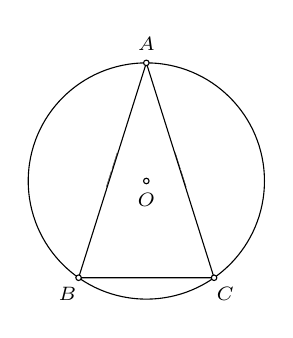
\begin{tikzpicture}[declare function={r=1.5;}]
	\path (0,0) coordinate (O);
	\foreach \goc/\bankinh/\t in {90/r/A,-125/r/B,-55/r/C}{
	\path (\goc:\bankinh) coordinate (\t);
	}
	\draw (O) circle (r) (A)--(B)--(C)--cycle;
	\path (A)--(B)node[sloped, midway]{\tiny ||};
	\path (A)--(C)node[sloped, midway]{\tiny ||};
	\foreach \t/\g in {A/90,B/-125,C/-55,O/-90}{
	\draw[fill=white] (\t) circle (1pt) node[shift={(\g:7pt)},font=\scriptsize]{$ \t $};
	}
	\end{tikzpicture}
	}
	\end{enumerate}
	}
\end{bt}
%%==========Bài 5
\begin{bt}%[9H3B7]
	Cho đường tròn $\left(O; R\right)$ và một dây cung $AB$.
	\begin{enumerate}
	\item Nếu biết $\text{sđ}\wideparen{AB} = 90^{\circ}$. Tính chu vi hình viên phân giới hạn bởi dây $AB$ và cung nhỏ $AB$.
	\item Nếu độ dài cung $AB$ là $\dfrac{5\pi R}{6}$. Tính số đo góc $\widehat{AOB}$.
	\end{enumerate}
	\loigiai{
	\begin{enumerate}
	\item Gọi $l$ là độ dài cung nhỏ $AB$. Do giả thiết suy ra $l = \dfrac{\pi\cdot R \cdot 90}{180} = \dfrac{\pi R}{2}$.\\
	Do tam giác $OAB$ vuông cân đỉnh $O$, theo định lí Py-ta-go ta có
	$$AB^2 = OA^2 + OB^2 = 2R^2\Rightarrow AB = R\sqrt{2}.$$
	Do đó chu vi hình viên phân giới hạn bởi dây $AB$ và cung nhỏ $AB$ là $$\dfrac{\pi R}{2} + \sqrt{2}R = \dfrac{\left(\pi + 2\sqrt{2}\right)R}{2}.$$	
	\item Gọi $n$ là số đo góc $\widehat{AOB}$. Theo công thức $l = \dfrac{\pi R n}{180}$ nên $\dfrac{5\pi R}{6} = \dfrac{\pi R n}{180}\Rightarrow n = 150$.\\
	Vậy số đo góc $\widehat{AOB} = 150^{\circ}$.
	\end{enumerate}
	}
\end{bt}
%%%%%%%% Quạt tròn
%%==========Bài 6
\begin{bt}
	Quan sát các hình sau.
	\begin{center}
	\begin{tabular}{cccc}
	\begin{tikzpicture}[>=stealth,line join=round,line cap=round,font=\footnotesize,scale=0.8]
	\def\r{2} 
	\path 
	(0,0) coordinate (O)
	(-10:\r) coordinate (M)
	(30:\r) coordinate (N)
	;
	\draw (O) circle(\r);
	\draw[fill=orange!50] (O)--(M) arc(-10:30:\r)--(N)--(O);
	\draw[orange] (M) arc(-10:30:\r);
	\draw (O)--(M) node[pos=0.5,below]{$2$ cm};
	;
	\draw[orange!50] (O)--(N);
	\node at ($(O)+(7:0.5)$){\tiny $40^{\circ}$};
	\foreach \x/\y in {O/90}
	\draw[fill=black] (\x) circle (1.1pt) + (\y:0.5cm);
	%	\draw pic[draw, angle radius=2mm, angle eccentricity=1.5]{right angle = C--A--B};
	\end{tikzpicture}
	& 
	\begin{tikzpicture}[>=stealth,line join=round,line cap=round,font=\footnotesize,scale=0.8]
	\def\r{2} 
	\path 
	(0,0) coordinate (O)
	(-10:\r) coordinate (M)
	(62:\r) coordinate (N)
	;
	\draw(O)--(M) arc(-10:62:\r)--(N)--(O);
	\draw[fill=orange!50] (O)--(N) arc(62:350:\r)--(M)--(O);
	\draw[orange!50] (N) arc(62:350:\r);
	\draw (O)--(M) node[pos=0.5,below]{$2$ cm};
	;
	\draw[orange!50] (O)--(N);
	\node at ($(O)+(20:0.6)$){\tiny $72^{\circ}$};
	\foreach \x/\y in {O/90}
	\draw[fill=black] (\x) circle (1.1pt) + (\y:0.5cm);
	%	\draw pic[draw, angle radius=2mm, angle eccentricity=1.5]{right angle = C--A--B};
	\end{tikzpicture}
	& 
	\begin{tikzpicture}[>=stealth,line join=round,line cap=round,font=\footnotesize,scale=0.8]
	\def\ra{2}
	\def\rb{0.55} 
	\path 
	(0,0) coordinate (O)
	(0:\rb) coordinate (M)
	(-90:\ra) coordinate (N)
	($(O)!0.7!(M)$) coordinate (x)
	($(x)+(0,0.7)$) coordinate (y)
	;
	%
	\draw[fill=orange!50] (O)circle(\ra);
	\draw[orange] (O)circle(\ra);
	\draw[fill=white] (O)circle(\rb);
	\draw[<->,red](O)--(N) node[pos=0.5,right]{$24$ cm};
	\draw[<-](x)--(y)node[above]{$6$ cm};
	\draw[<->,red] (O)--(M); %\draw[green!50] (O)--(M) node[pos=0.5,above]{$\tiny{ 2\, \text{cm}}$};
	%	;
	%	\draw[orange!50] (O)--(N);
	%	\node at ($(O)+(20:0.6)$){\tiny $72^{\circ}$};
	\foreach \x/\y in {O/90}
	\draw[fill=black] (\x) circle (1.1pt) + (\y:0.5cm);
	%	\draw pic[draw, angle radius=2mm, angle eccentricity=1.5]{right angle = C--A--B};
	\end{tikzpicture}
	& 
	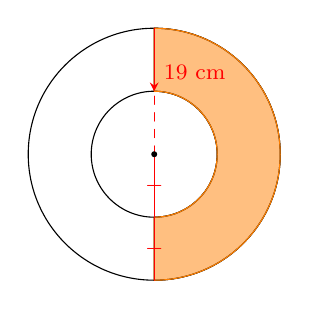
\begin{tikzpicture}[>=stealth,line join=round,line cap=round,font=\footnotesize,scale=0.8]
	\def\ra{2}
	\def\rb{1} 
	\path 
	(0,0) coordinate (O)
	(90:\rb) coordinate (M)
	(90:\ra) coordinate (N)
	(-90:\rb) coordinate (M')
	(-90:\ra) coordinate (N')
	;
	%
	\draw (O)circle(\ra);
	\draw (O)circle(\rb);
	\draw[fill=orange!50] (M')--(N')arc (-90:90:\ra)--(N)--(M) arc(90:-90:\rb)--cycle;
	\draw[orange] (M')--(N')arc (-90:90:\ra)--(N)--(M) arc(90:-90:\rb)--cycle;
	\draw[<-,red](M)--(N) node[pos=0.3,right]{$19$ cm};
	\draw[dashed,red](O)--(N);
	\draw[red] (O) edge node[midway, sloped, rotate=90, anchor=center] {$ - $}(M');
	\draw[red] (M')edge node[midway, sloped, rotate=90, anchor=center] {$ - $}(N');
	%	\draw[<->,red] (O)--(M); %\draw[green!50] (O)--(M) node[pos=0.5,above]{$\tiny{ 2\, \text{cm}}$};
	%	;
	%	\draw[orange!50] (O)--(N);
	%	\node at ($(O)+(20:0.6)$){\tiny $72^{\circ}$};
	\foreach \x/\y in {O/90}
	\draw[fill=black] (\x) circle (1.1pt) + (\y:0.5cm);
	%	\draw pic[draw, angle radius=2mm, angle eccentricity=1.5]{right angle = C--A--B};
	\end{tikzpicture}\\
	Hình a& Hình b& Hình c& Hình d\\
	\end{tabular}
	\end{center}
	\begin{enumerate}
	\item Tính diện tích phần được tô màu trong mỗi hình đó.
	\item Tính độ dài cung tròn được tô màu xanh ở mỗi hình a, b.
	\end{enumerate}
	\loigiai{
	\begin{enumerate}
	\item 
	\begin{itemize}
	\item Xét hình a.\\
	$S=\dfrac{\pi\cdot 2^2\cdot 40}{360}=\dfrac{4}{9}\pi\approx 1{,}4$ cm$^2$.
	\item Xét hình b.\\
	$S=\dfrac{\pi\cdot 2^2\cdot 72}{360}=\dfrac{4}{5}\pi\approx 2{,}5$ cm$^2$.
	\item Xét hình c.
	\\
	$S= \dfrac{1}{4} \pi\left(24^2-6^2\right)=135$ (cm$^2$).
	\item Xét hình d.
	\\
	$S= \dfrac{\tfrac{1}{4} \pi\left(38^2-19^2\right)}{2}=\dfrac{1083}{3}\approx 135{,}4$ (cm$^2$).
	\end{itemize}
	\item 
	\begin{itemize}
	\item Xét hình a.\\
	$S=\dfrac{\pi\cdot 2^2\cdot 320}{360}=\dfrac{32}{9}\pi\approx 11{,}2$ cm$^2$.
	\item Xét hình b.\\
	$S=\dfrac{\pi\cdot 2^2\cdot 288}{360}=\dfrac{16}{5}\pi\approx 10{,}1$ cm$^2$.
	\end{itemize}
	\end{enumerate}
	}
\end{bt}
%%==========Bài 7
\begin{bt}
	Tính diện tích các hình quạt tròn ứng với cung có số đo lần lượt là $30^{\circ}$; $90^{\circ}$; $120^{\circ}$ của hình tròn $(O ; 12 \mathrm{~cm})$.
	\loigiai{\begin{enumerate}
	\item Diện tích hình quạt tròn ứng với cung $ 30^\circ $ là $ \dfrac{\pi\cdot12^2\cdot30}{360} =12\pi \approx 37{,}7$ $\mathrm{(cm^2)}$.
	\item Diện tích hình quạt tròn ứng với cung $60^\circ $ là $ \dfrac{\pi\cdot12^2\cdot90}{360} =36\pi \approx 113{,}1$ $\mathrm{(cm^2)}$.
	\item Diện tích hình quạt tròn ứng với cung $ 30^\circ $ là $ \dfrac{\pi\cdot12^2\cdot120}{360} =48\pi \approx 150{,}8$ $\mathrm{(cm^2)}$.
	\end{enumerate}}
\end{bt}
%%==========Bài 8
\begin{bt}
	Tính diện tích các hình quạt tròn ứng với cung có độ dài lần lượt là $8 \mathrm{~cm}$, $15 \mathrm{~cm}$ của hình tròn $(O; 5 \mathrm{~cm})$.
	\loigiai{Vì diện tích hình quạt tròn tỉ lệ thuận với độ dài cung ứng với nó nên diện tích hình quạt tròn ứng với cung có độ dài là $ l $ được tính theo công thức là $S=\pi \mathrm{R}^2\cdot\dfrac{l}{2\pi \mathrm{R}}=\dfrac{\mathrm{R}l}{2} $.
	Khi đó:
	\begin{enumerate}
	\item Diện tích các hình quạt tròn ứng với cung có độ dài $ 8 \mathrm{~cm} $ là $ \dfrac{5\cdot8}{2}=20$ $ \mathrm{cm^2}$.
	\item Diện tích các hình quạt tròn ứng với cung có độ dài $ 15 \mathrm{~cm} $ là $ \dfrac{5\cdot15}{2}=37{,}5 $ $\mathrm{cm^2}$.
	\end{enumerate}}
\end{bt}
%%==========Bài 9
\begin{bt}
	Tính diện tích của hình quạt tròn bán kính $4$ cm, ứng với cung $36^{\circ}$.
	\loigiai{
	Diện tích của hình quạt tròn bán kính $4$ cm, ứng với cung $36^{\circ}$ là
	$S_{q}=\dfrac{36}{360}\cdot\pi\cdot4^{2}=1{,}6\pi~\left(\text{cm}^2\right).$
	}
\end{bt}
%%==========Bài 10
\begin{bt}
	\immini{
	Có hai chiếc bánh pizza hình tròn. Chiếc bánh thứ nhất có đường kính $16$ cm được cắt thành $6$ miếng đều nhau có dạng hình quạt tròn. Chiếc bánh thứ hai có đường kính $18$ cm được cắt thành $8$ miếng đều nhau có dạng hình quạt tròn. Hãy so sánh diện tích bề mặt của hai miếng bánh cắt ra từ chiếc bánh thứ nhất và thứ hai.
	}{
	
\includegraphics[scale=0.5]{images/9T5-15-H5.18.png}
	}
	\loigiai{
	Diện tích miếng bánh được cắt ra từ chiếc bánh thứ nhất là
	\[S_1=\dfrac{360}{360}\cdot\pi\cdot16^{2}:6=\dfrac{128\pi}{3}~\left(\text{cm}^2\right).\]
	Diện tích miếng bánh được cắt ra từ chiếc bánh thứ hai là
	\[S_2=\dfrac{360}{360}\cdot\pi\cdot18^{2}:8=\dfrac{81\pi}{2}~\left(\text{cm}^2\right).\]
	Vì $\dfrac{128\pi}{3}>\dfrac{81\pi}{2}$ nên diện tích miếng bánh được cắt ra từ chiếc bánh thứ nhất lớn hơn diện tích miếng bánh được cắt ra từ chiếc bánh thứ hai.
	}
\end{bt}
%%==========Bài 11
\begin{bt}
	Khi đóng đáy thuyền cho những con thuyền vượt biển, người Vikings sử dụng hai loại nêm nêm góc và nêm cong (lần lượt tô màu xanh, màu đỏ trong Hình a). Mặt cắt $A B C D$ của nêm góc có dạng hai tam giác vuông $O A E$, $O D E$ bằng nhau với cạnh huyền chung và bỏ đi hình quạt tròn $O B C$ (Hình b), được làm từ những thân cây mọc thẳng. Mặt cắt $M N P Q$ của nêm cong có dạng một phần của hình vành khuyên (Hình c), được làm từ những thân cây cong. Kích thước của nêm cong được cho như ở Hình c.
	\begin{center}
	\begin{tabular}{ccc}
	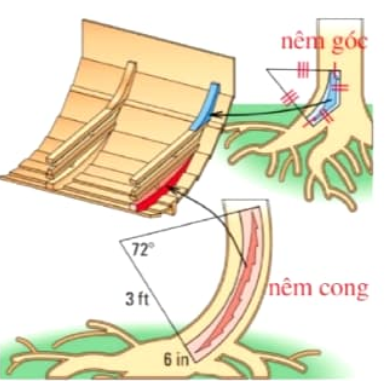
\includegraphics[scale=0.7]{images/images-9C5-5/hinh89-bt4-Bai3-Dtichhinhquat-vanhkhuyen.PNG}
	&
	\begin{tikzpicture}[>=stealth,line join=round,line cap=round,font=\footnotesize,scale=0.8]
	\def\r{3.5} 
	\path 
	(0,-0.5) coordinate (O)
	(-115:\r) coordinate (B)
	(-65:\r) coordinate (C)
	(-90:\r) coordinate (N)
	($(N)!1!180:(O)$) coordinate (x)
	($(B)!0.3!180:(O)$) coordinate (A)
	($(C)!0.3!180:(O)$) coordinate (D)
	($(A)!0.5!-90:(O)$) coordinate (y)
	($(D)!0.3!90:(O)$) coordinate (z)
	(intersection of A--y and O--x) coordinate (M)
	;
	\draw[fill=cyan!50!blue] (B) arc(-115:-65:\r)--(C)--(D)--(M)--(A)--(B);
	\draw[dashed,blue] (B)--(O)--(C) (O)--(M);
	\foreach \x/\y in {O/90,A/190,B/180,C/0,D/0,M/-90,N/-65}
	\draw[fill=black] (\x) circle (1.1pt) + (\y:0.5cm) node{$\x$};
	\draw pic[draw, angle radius=2mm, angle eccentricity=1.5]{right angle = M--A--B};
	\draw pic[draw, angle radius=2mm, angle eccentricity=1.5]{right angle = C--D--M};
	\draw (B)edge node[midway, sloped, rotate=90, anchor=center] {$ - $}(A);
	\draw (C)edge node[midway, sloped, rotate=90, anchor=center] {$ - $}(D);
	\draw (A)edge node[midway, sloped, rotate=90, anchor=center] {$ = $}(M);
	\draw (D)edge node[midway, sloped, rotate=90, anchor=center] {$ = $}(M);
	\end{tikzpicture}
	&
	\begin{tikzpicture}[>=stealth,line join=round,line cap=round,font=\footnotesize,scale=0.8]
	\def\r{3.5}
	\def\ra{4.2} 
	\path 
	(0,0) coordinate (I)
	(-126:\r) coordinate (N)
	(-54:\r) coordinate (P)
	(-126:\ra) coordinate (M)
	(-54:\ra) coordinate (Q)
	;
	\draw[dashed,blue] (N)--(I);
	\draw[dashed,blue] (I)--(P)node[pos=0.5,right]{$3$ ft};
	\draw[blue] (P)--(Q) node[pos=0.5,right] {$6$ in};
	\draw[fill=red!50] (N) arc(-126:-54:\r)--(P)--(Q)--(Q) arc(-54:-126:\ra)--(M)--(N);
	\node at ($(I)+(-90:0.8)$){$72^{\circ}$};
	\foreach \x/\y in {I/90,N/180,M/180,P/90,Q/-20}
	\draw[fill=black] (\x) circle (1.1pt) + (\y:0.5cm) node{$\x$};
	\end{tikzpicture}\\
	Hình a& Hình b& Hình c
	\end{tabular}
	\end{center}	
	\begin{enumerate}
	\item Diện tích của nêm cong là bao nhiêu centimét vuông (lấy $1\text{ft}=30$ cm, $1 \text{in} =2{,}54$ cm, $\pi=3{,}14$ và làm tròn kết quả đến hàng đơn vị)?
	\item Cần phải biết những kích thước nào của nêm góc để tính được diện tích của nêm đó?
	\end{enumerate}
	\loigiai{
	\begin{enumerate}
	\item Diện tích của nêm cong là \\
	$\dfrac{1}{5}\cdot \dfrac{1}{4}\cdot 3{,14} \cdot 6\cdot 2{,}54\approx 2{,}4$ cm$^2$.
	\item Cần phải biết $OA$, $OB$ và $OM$ thì tính được diện tích của nêm.\\ Khi đó $S_{\text{(nêm)}}=2\left(S_{\triangle OAM}-S_{\text{quạt} BON}\right).$
	\end{enumerate}
	}
\end{bt}
%%==========Bài 12
\begin{bt}
	Tính diện tích hình vành khuyên giới hạn bởi hai đường tròn $({O} ; 9 \mathrm{~cm})$ và $({O} ; 12 \mathrm{~cm})$.
	\loigiai{Diện tích hình vành khuyên là $ S=\pi(12^2-9^2)=63\pi\approx 197{,}92$ $\mathrm{cm^2} $.}
\end{bt}
%%==========Bài 13
\begin{bt}
	Tính diện tích hình vành khuyên nằm giữa hai đường tròn đồng tâm có bán kính là $6$ cm và $4$ cm.
	\loigiai{
	Diện tích hình vành khuyên nằm giữa hai đường tròn đồng tâm có bán kính là $6$ cm và $4$ cm là
	\[S_{v}=\pi\left(6^{2}-4^{2}\right)=20\pi~\left(\text{cm}^2\right).\]
	}
\end{bt}
%%==========Bài 14
\begin{bt}
	\immini{Hình bên mô tả mặt cắt của một chiếc đèn led có dạng hai hình vành khuyên màu trắng với bán kính các đường tròn lần lượt là $15$ cm, $18$ cm, $21$ cm, $24$ cm. Tính diện tích hai hình vành khuyên đó.}
	{
\includegraphics[scale=0.8]{images/images-9C5-5/hinh87-bt2-C5-Bai5-Dodaicungtron}}
	\loigiai{
	$S_1= \dfrac{1}{4} \pi\left(18^2-15^2\right)=\dfrac{99\pi}{4}\approx 77{,}8$ (cm$^2$).\\
	$S_2= \dfrac{1}{4} \pi\left(24^2-21^2\right)=\dfrac{135\pi}{4}\approx 106$ (cm$^2$).
	}
\end{bt}
%%==========Bài 15
\begin{bt}
	\immini{
	Một chiếc quạt giấy khi xoè ra có dạng nửa hình tròn bán kính $2{,}2$ dm như hình bên. Tính diện tích phần giấy của chiếc quạt, biết rằng khi gấp lại, phần giấy có chiều dài khoảng $1{,}6$ dm (làm tròn kết quả đến hàng phần trăm của dm$^2$).
	}{
	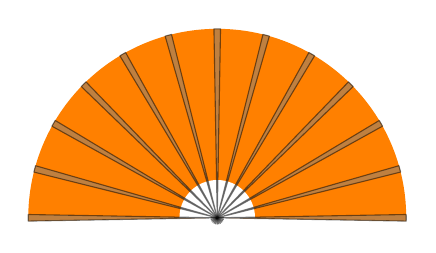
\begin{tikzpicture}[>=stealth,line join=round,line cap=round,font=\footnotesize,scale=0.8]
	\def\r{0.1};\def\R{3};
	\fill[orange] (0,0)--(-1:\R)arc(-1:181:\R)--cycle;
	\fill[white] (0:0.2*\R)arc(0:180:0.2*\R)--cycle;
	\draw (0,0) coordinate (O);
	\foreach \x in {0,15,...,180}{\draw[fill=gray,opacity=0.5] (180+\x-1:\r)--(\x-1:\R)arc(\x-1:\x+1:\R)--(180+\x+1:\r);}
	\end{tikzpicture}
	}
	\loigiai{
	Phần giấy của chiếc quạt là một hình vành khuyên với bán kính đường tròn lớn là $2{,}2$ dm và bán kính đường tròn nhỏ là $2{,}2-1{,}6=0{,}6$ dm.\\
	Vậy diện tích phần giấy của chiếc quạt là
	\[S=\dfrac{1}{2}\cdot\pi\cdot\left[(2{,}2)^{2}-(0{,}6)^{2}\right]\approx7{,}04~\left(\text{dm}^2\right).\]
	}
\end{bt}
%%==========Bài 16
\begin{bt}
	\immini{Tính diện tích hình viên phân giới hạn bởi dây cung có độ dài là $55$ cm và cung có số đo là $95^{\circ}$.}	{\begin{tikzpicture}[line join=round, line cap=round,|| mark/.style={postaction=decorate,decoration={markings,
	mark=at position #1 with {\draw[line cap=round,mark segment] (-1pt,-2pt) -- (-1pt,2pt);
	\draw[line cap=round,mark segment] (1pt,-2pt) -- (1pt,2pt);
	}}},mark segment/.style={thick},scale=0.9]
	\coordinate (I) at (0,0);
	\coordinate (N) at (0:2.3cm);
	\coordinate (M) at (95:2.3cm);
	\coordinate (E) at (0:0.2cm);
	\coordinate (F) at (0:0cm);
	\coordinate (G) at (95:0.2cm);
	\coordinate (H) at ($(M)!0.5!(N)$);
	\coordinate (d1) at ($(N)!1.5!(M)$);
	\coordinate (d2) at ($(M)!1.5!(N)$);
	\node[below] at (0:1cm) {$5\, \text{cm}$};
	\draw[thick,red] (I) circle[radius=2.3cm];
	\draw (M)--(I)--(N)--(M);
	\draw (I)--(H);
	\draw pic [draw,black,angle radius=2mm] {right angle=M--H--I};
	\draw pic["$95^{\circ}$",draw=blue,double,-,angle eccentricity=1.5, angle radius=0.5cm] {angle=E--F--G};
	\draw[|| mark=0.5] (H)--(M);
	\draw[|| mark=0.5] (H)--(N);
	\foreach \x/\g in {M/110,N/70,H/90,I/-90}
	\draw[fill=white] (\x) circle (1.5pt)+(\g:3mm) node {$\x$};
	\end{tikzpicture}}
	\loigiai{Diện tích hình quạt tròn giới hạn bởi $IM$, $IN$ và cung nhỏ $MN$ là 
	$S_{\text{quạt}} = \dfrac{\pi\cdot 5^{2}\cdot 95}{360} = \dfrac{475 \pi}{72} \, (\mathrm{cm}^{2}).$\\
	Diện tích tam giác $MIN$ là $S_{MIN} = \dfrac{1}{2}\cdot5\cdot5\cdot\sin 95^{\circ} \, (\mathrm{cm}^{2})$.\\
	Diện tích của hình viên phân giới hạn bởi dây cung $MN$ là 
	$S = S_{\text{quạt}} - S_{MIN} \approx 12{,}2\,(\mathrm{cm}^2).$
	}
\end{bt}
%%==========Bài 17
\begin{bt}
	Hình dưới mô tả mặt cắt của một khung gỗ có dạng ghép của năm hình: hai nửa đường tròn đường kính $2$ cm; hai hình chữ nhật kích thước $2$ cm $ \times 8$ cm; một phần tư hình vành khuyên giới hạn bởi hai đường tròn cùng tâm có bán kính lần lượt là $4$ dm và $6$ dm. Tính diện tích của mặt cắt của khung gỗ đó.
	\begin{center}
	\begin{tabular}{ccc}
	\begin{tikzpicture}[>=stealth,line join=round,line cap=round,font=\footnotesize,scale=0.8]
	\def\r{0.4} 
	\def\rn{1.2}
	\def \rl{2}
	\path 
	(0,0) coordinate (O)
	(90:\r) coordinate (M)
	(270:\r) coordinate (N)
	($(M)+(2.8,0)$) coordinate (P)
	($(N)+(2.8,0)$) coordinate (Q)
	($(P)+(0,0.6)$) coordinate (I)
	(P) arc (-90:0:\rn)coordinate (P')
	(Q) arc (-90:0:\rl)coordinate (Q')
	($(P')+(0,2.8)$) coordinate (M')
	($(Q')+(0,2.8)$) coordinate (N')
	($(M')!0.5!(N')$) coordinate (O')
	;
	\draw (M') arc (180:0:\r);
	\draw (P)--(M)arc (90:270:\r)--(N)--(Q);
	\draw (P) arc (-90:0:\rn);
	\draw(Q) arc (-90:0:\rl); 
	\draw (P')--(M') (Q')--(N');
	\foreach \x/\y in {O/90,O'/90}
	\draw[fill=red] (\x) circle (1.1pt) + (\y:0.5cm);
	\draw[fill=orange!50] (M) arc (90:270:\r) --(N)--(M);
	\draw[fill=orange!50] (M') arc (180:0:\r) --(N')--(M');
	\draw[<->](M)--(N)node[pos=0.5,right]{$2$cm};
	\draw[<->](M')--(N')node[pos=0.5,below]{$2$cm} ;
	\end{tikzpicture}
	& \begin{tikzpicture}[>=stealth,line join=round,line cap=round,font=\footnotesize,scale=0.8]
	\def\r{0.4} 
	\def\rn{1.2}
	\def \rl{2}
	\path 
	(0,0) coordinate (O)
	(90:\r) coordinate (M)
	(270:\r) coordinate (N)
	($(M)+(2.8,0)$) coordinate (P)
	($(N)+(2.8,0)$) coordinate (Q)
	($(P)+(0,0.6)$) coordinate (I)
	(P) arc (-90:0:\rn)coordinate (P')
	(Q) arc (-90:0:\rl)coordinate (Q')
	($(P')+(0,2.8)$) coordinate (M')
	($(Q')+(0,2.8)$) coordinate (N')
	($(M')!0.5!(N')$) coordinate (O')
	($(M)+(0,0.3)$) coordinate (x)
	($(P)+(0,0.3)$) coordinate (y)
	($(N')+(0.3,0)$) coordinate (x')
	($(Q')+(0.3,0)$) coordinate (y')
	;
	\draw (M') arc (180:0:\r);
	\draw (P)--(M)arc (90:270:\r)--(N)--(Q);
	\draw (P) arc (-90:0:\rn);
	\draw(Q) arc (-90:0:\rl); 
	\draw (P')--(M') (Q')--(N');
	\draw[fill=orange!50](M)--(N)--(Q)--(P)--(M);
	\draw[fill=orange!50](M')--(N')--(Q')--(P')--(M');
	\draw[<->](M)--(N)node[pos=0.5,right]{$2$ cm};
	\draw[<->](P')--(Q')node[pos=0.7,below]{$2$ cm} ; 
	\draw[<->](x)--(y)node[pos=0.5,above]{$8$ cm};
	\draw[<->](x')--(y')node[pos=0.5,right]{$8$ cm} ; 
	\draw[dashed] (M)--(x) (Q)--(y) (N')--(x') (P')--(y')(M')--(N');
	\end{tikzpicture}
	&\begin{tikzpicture}[>=stealth,line join=round,line cap=round,font=\footnotesize,scale=0.8]
	\def\r{0.4} 
	\def\rn{1.2}
	\def \rl{2}
	\path 
	(0,0) coordinate (O)
	(90:\r) coordinate (M)
	(270:\r) coordinate (N)
	($(M)+(2.8,0)$) coordinate (P)
	($(N)+(2.8,0)$) coordinate (Q)
	($(P)+(0,0.6)$) coordinate (I)
	(P) arc (-90:0:\rn)coordinate (P')
	(Q) arc (-90:0:\rl)coordinate (Q')
	($(P')+(0,2.8)$) coordinate (M')
	($(Q')+(0,2.8)$) coordinate (N')
	($(M')!0.5!(N')$) coordinate (O')
	($(P')!4!180:(Q')$) coordinate (x)
	($(P)!4!180:(Q)$) coordinate (y)
	(intersection of P'--x and P--y) coordinate (I)
	($(I)+(0,.5)$) coordinate (u)
	($(P')+(0,.5)$) coordinate (v)
	($(I)+(-0.3,0)$) coordinate (u')
	($(Q)+(-0.3,0)$) coordinate (v')
	;
	\draw (M') arc (180:0:\r);
	\draw (P)--(M)arc (90:270:\r)--(N)--(Q);
	\draw (P) arc (-90:0:\rn);
	\draw(Q) arc (-90:0:\rl); 
	\draw (P')--(M') (Q')--(N');
	%\draw[fill=orange!50] (M')--(N')arc (-90:90:\ra)--(N)--(M) arc(90:-90:\rb)--cycle;
	\draw[fill=orange!50] (P)--(Q)arc (-90:0:\rl)--(Q')--(P') arc(0:-90:\rn)--cycle;
	%	\draw (P)--(Q)arc (-90:0:\rl)--(Q')--(P') arc (-90:0:\rn)--(Q);
	\draw[<->](u)--(v)node[pos=0.5,above]{$4$ cm};
	\draw[<->](u')--(v')node[pos=0.5,left]{$6$ cm} ; 
	\draw (Q)--(P)--(I)--(P')--(Q');
	\draw[dashed](I)--(u')(I)--(u);
	\draw pic[draw, angle radius=2mm, angle eccentricity=1.5]{right angle = P--I--P'};
	\end{tikzpicture}\\
	\end{tabular}
	\end{center}
	\loigiai{
	Diện tích mặt cắt $S=2\cdot \dfrac{1}{2}\cdot \pi\cdot 1^2+2\cdot 2\cdot 8+\dfrac{1}{4}\pi (6^2-4^2)\approx 50{,}85$ cm$^2$.
	}
\end{bt}
%%==========Bài 18
\begin{bt}%[9H3K7]
	Cho đường tròn $\left(O; R\right)$.
	\begin{enumerate}
	\item Tính $\widehat{AOB}$ biết độ dài cung $AB$ là $\dfrac{\pi R}{3}$.
	\item Trên cung lớn $AB$ lấy điểm $C$ sao cho $\triangle AOC$ vuông cân tại $O$. Tính độ dài $\wideparen{AC}$, $\wideparen{BC}$ lớn.
	\end{enumerate}
	\loigiai{
	\begin{enumerate}
	\item Theo công thức $l = \dfrac{\pi R n}{180}$ nên $\dfrac{\pi R}{3} = \dfrac{\pi R n}{180}\Rightarrow n = 60$.\\
	Vậy $n^{\circ} = 60^{\circ}$ hay $\widehat{AOB} = 60^{\circ}$.
	\item Do giả thiết suy ra $\text{sđ}\wideparen{AC} = 90^{\circ}$ nên độ dài $\wideparen{AC}$ là $\dfrac{\pi\cdot R\cdot 90}{180} = \dfrac{\pi R}{2}$.\\
	Mặt khác số đo cung lớn $BC$ là $360^{\circ} - 60^{\circ} - 90^{\circ}= 210^{\circ}$.\\
	Khi đó độ dài $\wideparen{BC}$ là $\dfrac{\pi\cdot R\cdot 210}{180} = \dfrac{7\pi R}{6}$.
	\end{enumerate}
	}
\end{bt}
%%==========Bài 19
\begin{bt}%[9H3K7]
	Cho đường tròn đường tròn đường kính $AB$. Vẽ dây $CD$ vuông góc với $AB$ tại $M$. Giả sử $AM = 1\, \mathrm{cm}$, $CD = 2\sqrt{3}\, \mathrm{cm}$.
	\begin{listEX}[2]
	\item Tính độ dài đường tròn.
	\item Tính độ dài cung $\wideparen{CAD}$.
	\end{listEX}
	\loigiai{
	\immini
	{	\begin{enumerate}
	\item Do giả thiết suy ra $\triangle ABC$ vuông tại $C$. Áp dụng hệ thức lượng trong $\triangle ABC$, ta có $CM^2 = AM\cdot MB$.\\
	Vì $CD\perp AB$ nên $MC = MD = \dfrac{CD}{2} = \sqrt{3}\, \left(\mathrm{cm}\right)$ do đó $MB = 3\, \left(\mathrm{cm}\right)$ và $AB = AM + MB = 4\, \left(\mathrm{cm}\right)$.\\
	Khi đó độ dài đường tròn là $2\pi R = 4\pi\, \left(\mathrm{cm}\right)$.
	\item Áp dụng định lí Py-ta-go trong $\triangle AMC$ vuông, ta có 
	$AC^2 = AM^2 + CM^2 = 1 + 3 = 4\Rightarrow AC = 2\, \left(\mathrm{cm}\right)$. Suy ra $OA = OC = AC$ hay $\triangle AOC$ là tam giác đều nên $\widehat{AOC} = 60^{\circ}$.\\
	\end{enumerate}
	}
	{\begin{tikzpicture}[line join = round, line cap = round,>=stealth,scale=0.7]
	\clip (-3.5, -3.5) rectangle (3.5,3.5);
	\tkzDefPoints{0/0/O}
	\def \R{3}; %Bán kính
	\tkzDefShiftPoint[O](0:\R){B}
	\tkzDefShiftPoint[O](-180:\R){A}
	\tkzDefShiftPoint[O](118:\R){C}
	\tkzDefLine[perpendicular=through C](A,B) \tkzGetPoint{c}
	\tkzInterLL(A,B)(C,c) \tkzGetPoint{M}
	\tkzInterLC[R](C,c)(O,\R ) \tkzGetPoints{x}{D}
	\draw (O) circle (\R);
	\tkzLabelPoints[below left](M)
	\tkzLabelPoints[left](A)
	\tkzLabelPoints[below right](O)
	\tkzLabelPoints[right](B)
	\tkzLabelPoints[below](D)
	\tkzLabelPoints[above](C)
	\tkzDrawSegments(A,B A,C C,B C,D O,C O,D)
	\tkzDrawPoints[fill=black](O,A,B,C,D,M)
	\tkzMarkRightAngles(A,M,C A,C,B)
	\end{tikzpicture}	
	}
	Mà $\widehat{COD} = 2\widehat{AOC} = 2\cdot 60^{\circ} = 120^{\circ}$.
	Khi đó độ dài cung $\wideparen{CAD}$ là $\dfrac{\pi\cdot R\cdot n}{180} = \dfrac{\pi\cdot R\cdot 120}{180} = \dfrac{2\pi R}{3}$.	
	}
\end{bt}
%%==========Bài 20
\begin{bt}%[9H3B7]
	Tính chu vi hình vẽ bên, biết $OA = 4\, \mathrm{cm}$.
	\loigiai{
	\immini
	{Do giả thiết suy ra $OA = OB = 4\, \mathrm{cm}$ và $AB = 2OA = 8\, \mathrm{cm}$.\\
	Gọi $C$ là chu vi hình khi đó 
	$$C = \dfrac{1}{2}\cdot\dfrac{\pi\cdot 4\cdot 180}{180} + \dfrac{1}{2}\cdot\dfrac{\pi\cdot 4\cdot 180}{180} + \dfrac{1}{2}\cdot\dfrac{\pi\cdot 8\cdot 180}{180} = 8\pi.$$
	Vậy chu vi hình là $8\pi$.
	}
	{\begin{tikzpicture}[line join = round, line cap = round,>=stealth,scale=1]
	\tkzDefPoints{0/0/A}
	\tkzDefShiftPoint[A](0:4){B}
	\tkzDefMidPoint(A,B)\tkzGetPoint{O}
	\tkzDefMidPoint(A,O)\tkzGetPoint{I}
	\tkzDefMidPoint(B,O)\tkzGetPoint{J}	
	\pgfresetboundingbox
	\tkzDrawSegments[dashed](A,B)
	\tkzDrawPoints[fill=black](A,B,O)
	\tkzLabelPoints[left](A)
	\tkzLabelPoints[right](B)
	\tkzLabelPoints[below left](O)
	\tkzDrawArc[rotate,color = black, line width = 0.6pt](J,B)(-180)
	\tkzDrawArc[rotate,color = black, line width = 0.6pt](O,B)(180)
	\tkzDrawArc[rotate,color = black, line width = 0.6pt](I,O)(180)
	\end{tikzpicture}
	}
	}
\end{bt}
%%==========Bài 21
\begin{bt}%[9H3K1]
	Cho tam giác $ABC$ nội tiếp đường tròn $\left(O; R\right)$. Biết rằng $\dfrac{\text{sđ}\wideparen{BC}}{1} = \dfrac{\text{sđ}\wideparen{CA}}{2}= \dfrac{\text{sđ}\wideparen{AB}}{3}$. Gọi $a$, $b$, $c$ lần lượt là độ dài các đường tròn đường kính $BC$, $CA$, $AB$.
	Chứng minh rằng \[\dfrac{a}{1} = \dfrac{b}{\sqrt{3}} = \dfrac{c}{2}.\]
	\loigiai{
	\immini
	{Đặt $x = \text{sđ}\wideparen{BC}$, $y = \text{sđ}\wideparen{CA}$ và $z = \text{sđ}\wideparen{AB}$.\\
	Do giả thiết $\dfrac{x}{1} = \dfrac{y}{2} = \dfrac{z}{3} = \dfrac{x + y + z}{1 + 2 + 3}$.\\
	Mà $x + y + z = 360^{\circ}$ do đó $\dfrac{x}{1} = \dfrac{y}{2} = \dfrac{z}{3} = \dfrac{360^{\circ}}{6} = 60^{\circ}$.
	\begin{itemize}
	\item Khi $\dfrac{x}{1} = 60^{\circ}$ suy ra $x = 60^{\circ}$.
	\item Khi $\dfrac{y}{2} = 60^{\circ}$ suy ra $y = 2\cdot 60^{\circ} = 120^{\circ}$.
	\item Khi $\dfrac{z}{3} = 60^{\circ}$ suy ra $z = 3\cdot 60^{\circ} = 180^{\circ}$.
	\end{itemize}
	}
	{\begin{tikzpicture}[line join = round, line cap = round,>=stealth,scale=0.8]
	\tkzDefPoints{0/0/O}
	\def \R{3}; %Bán kính
	\draw (O) circle (\R);
	\tkzDefShiftPoint[O](0:\R){A}
	\tkzDefShiftPoint[O](120:\R){C}
	\tkzDefShiftPoint[O](-180:\R){B}
	\tkzLabelPoints[above](C)
	\tkzLabelPoints[left](B)
	\tkzLabelPoints[right](A)
	\tkzLabelPoints[below](O)
	\tkzDrawPoints[fill=black](O,A,B,C)
	\tkzDrawSegments(A,B A,C B,C)
	\tkzMarkRightAngles(B,C,A)
	\end{tikzpicture}	
	}
	\noindent Nên $\triangle ABC$ có $\widehat{BAC} = 90^{\circ}$, $\widehat{CBA} = 60^{\circ}$ và $\widehat{BAC} = 30^{\circ}$. Suy ra $AB = 2R$, $CB = R$ và $AC = \sqrt{3}R$.\\
	Khi đó $a = \pi R$, $b = \sqrt{3}\pi R$ và $c = 2\pi R$ suy ra $\dfrac{a}{1} = \dfrac{b}{\sqrt{3}} = \dfrac{c}{2}$.
	}
\end{bt}
%%==========Bài 22
\begin{bt}%[9H3K7]
	Cho tam giác $ABC$ đều nội tiếp đường tròn $\left(O; 6\, \mathrm{cm}\right)$. 
	Vẽ bên ngoài tam giác $ABD$ vuông cân tại $D$. Các đường thẳng $AD$, $DB$ lần lượt cắt đường tròn $\left(O\right)$ tại $M$, $N$. Tính độ dài cung nhỏ $AM$, $BN$, $MN$ và $MC$.	
	\loigiai{
	\immini
	{Ta có $\widehat{ACB} = \dfrac{1}{2}\text{sđ}\wideparen{AB}$ mà $\widehat{ACB} = 60^{\circ}$ suy ra $\text{sđ}\wideparen{AB} = 120^{\circ}$.\\
	Tương tự $\widehat{MAB} = \dfrac{1}{2}\text{sđ}\wideparen{MB}$ mà $\widehat{MAB} = 45^{\circ}$ suy ra $\text{sđ}\wideparen{MB} = 90^{\circ}$.\\
	Suy ra $\text{sđ}\wideparen{MA} = \text{sđ}\wideparen{AB} - \text{sđ}\wideparen{MB} = 120^{\circ} - 90^{\circ} = 30^{\circ}$.\\
	Gọi $l$ là độ dài cung $\wideparen{MA}$, ta có
	$$l = \dfrac{\pi R n}{180} = \dfrac{\pi\cdot 6\cdot 30}{180} = \pi.$$
	Dễ thấy độ dài cung $\wideparen{NB}$ bằng $\pi$.\\
	}
	{\begin{tikzpicture}[line join = round, line cap = round,>=stealth,scale=0.7]
	\tkzDefPoints{0/0/O}
	\def \R{3}; %Bán kính
	\draw (O) circle (\R);
	\tkzDefShiftPoint[O](90:\R){A}
	\tkzDefShiftPoint[O](-30:\R){C}
	\tkzDefShiftPoint[O](-150:\R){B}
	\tkzDefTriangle[two angles = 45 and 45](B,A)\tkzGetPoint{D}
	\tkzInterLC[R](D,A)(O,\R )\tkzGetPoints{x}{M}
	\tkzInterLC[R](D,B)(O,\R ) \tkzGetPoints{N}{x}
	\tkzLabelPoints[above](A,M)
	\tkzLabelPoints[left](B,D,N)
	\tkzLabelPoints[right](C)
	\tkzLabelPoints[above right](O)
	\tkzDrawPoints[fill=black](O,A,B,C,D,M,N)
	\tkzDrawSegments(A,B A,C B,C D,A D,B O,A O,B O,C O,M O,N)
	\tkzMarkRightAngles(B,D,A)
	\end{tikzpicture}	
	}\noindent
	Mặt khác $\text{sđ}\wideparen{MN} = \text{sđ}\wideparen{AB} - \text{sđ}\wideparen{MA} - \text{sđ}\wideparen{NB}= 120^{\circ} - 30^{\circ} - 30^{\circ} = 60^{\circ}$.\\
	Khi đó, gọi $l'$ là độ dài cung $MN$ ta có $l' = \dfrac{\pi R n}{180} = \dfrac{\pi\cdot 6\cdot 60}{180} = 2\pi.$\\
	Gọi $l''$ là độ dài cung $AC$ suy ra $l'' = \dfrac{\pi R n}{180} = \dfrac{\pi\cdot 6\cdot 120}{180} = 4\pi.$\\
	Do đó độ dài cung $MC$ bằng $\pi + 4\pi = 5\pi$.
	}
\end{bt}
%%==========Bài 23
\begin{bt}%[9H3B10]
	Cho hình tròn ($O$; $3$ cm) và điểm $M$ nằm ngoài đường tròn. Qua $M$ kẻ tiếp tuyến $MA$, $MB$ tới đường tròn. Biết $\widehat{AMB}=60^\circ$. Tính diện tích hình giới hạn bởi $MA$, $MB$ và cung nhỏ $AB$.
	\loigiai
	{
	\immini{	Ta có $\widehat{AMB}=60^\circ$ nên $\widehat{AOB}=120^\circ$.\\
	$MA$, $MB$ là tiếp tuyến của đường tròn nên \[\widehat{O_1}=\widehat{O_2}=\dfrac{1}{2}\widehat{AOB}=60^\circ.\]
	Ta có $MA=AO \cdot \tan \widehat{AOM}=3\sqrt{3}$ (cm).
	Diện tích tứ giác $MAOB$ là
	\begin{align*}
	S_1 & = \;2 \cdot S_{MAO}=2 \cdot \frac{1}{2} \cdot MA \cdot AO\\
	&=\; 3\sqrt3 \cdot 3 = 9\sqrt{3}\; \text{(cm$^2$)}.
	\end{align*}
	}
	{\begin{tikzpicture}[line join = round, line cap = round,>=stealth,scale=0.75]
	\tkzDefPoints{0/0/O}
	\def\bankinh{2}
	\tkzDefShiftPoint[O](0:\bankinh){C}
	\tkzDefShiftPoint[O](180:4){M}
	\tkzDefTangent[from=M](O,C) \tkzGetPoints{B}{A}
	\tkzDefShiftPoint[O](150:0.5){c}
	\tkzDefShiftPoint[O](210:0.5){d}
	\pgfresetboundingbox
	\tkzDrawCircle[radius](O,C)
	\tkzDrawSegments(M,A M,B O,A O,B O,M)
	\tkzDrawPoints[fill=black](A,B,O,M)
	\tkzLabelPoints[above](B)
	\tkzLabelPoints[right](O)
	\tkzLabelPoints[below](A)
	\tkzLabelPoints[left](M)
	\tkzMarkRightAngles[size=0.2](O,A,M O,B,M)
	\draw (c) node {$1$};
	\draw (d) node {$2$};
	\end{tikzpicture}}
	\noindent Diện tích hình quạt $OAB$ là:
	$$S_\text{q} = \frac{\pi R^2 n}{360}=\frac{\pi \cdot 9 \cdot 120}{360}=3\pi \; \text{(cm$^2$)}.$$
	Vậy diện tích hình giới hạn bởi $MA$, $MB$ và cung nhỏ $AB$ là 
	$$S=S_1-S_\text{q}=9\sqrt{3} -3\pi = 3\left(3\sqrt{3} - \pi \right) \; \text{(cm$^2$)}.$$
	}
\end{bt}
%%==========Bài 24
\begin{bt}%[9H3B10]
	\immini{Cho hình vẽ. Biết rằng $\widehat{AOB}=90^\circ$; $OA=OB=6$cm. Tính diện tích phần tô đen.}
	{\begin{tikzpicture}[line join = round, line cap = round,>=stealth,scale=1]
	\tkzDefPoints{0/0/O}
	\tkzDefShiftPoint[O](90:3){A}
	\tkzDefShiftPoint[O](0:3){B}
	\tkzDefMidPoint(O,B)\tkzGetPoint{M}
	\pgfresetboundingbox
	\tkzDrawPoints[fill=black](O,A,B,M)
	\tkzDrawSegments(O,A O,B)
	\tkzDrawSector[rotate,fill = gray!50,line width=0.6pt](O,B)(90)
	\tkzDrawSector[rotate,fill = white,line width=0.6pt](M,B)(180)
	\fill (O) circle (1.5pt);
	\fill (M) circle (1.5pt);
	\fill (B) circle (1.5pt);
	\tkzLabelPoints[right](B)
	\tkzLabelPoints[left](A)
	\tkzLabelPoints[below](O,M)
	\tkzMarkRightAngles[size=0.2](A,O,B)
	\end{tikzpicture}	}
	\loigiai
	{
	Diện tích hình quạt $(OAB)$ là
	$$S_1=\frac{\pi R^2n}{360}=\frac{\pi \cdot 6^2 \cdot 90}{360}=9\pi \; \text{(cm$^2$)}.$$
	Diện tích nửa hình tròn đường kính $OB$ là
	$$S_2=\frac{1}{2}\pi \cdot 3^2 =\frac{9}{2}\pi \; (cm^2).$$
	Vậy diện tích phần tô đen là $S_1-S_2=9\pi - \dfrac{9}{2}\pi = 4,5\pi$ (cm$^2$).
	}
\end{bt}
%%==========Bài 25
\begin{bt}%[9H3B10]
	Trên đường tròn ($O$; $R$) có hai điểm $A$, $B$ sao cho $sđ \stackrel\frown{AB} = 60^\circ$; Trên ($O'$; $R'$) có hai điểm $C$, $D$ sao cho $sđ \stackrel\frown{CD} = 45^\circ$. Biết rằng hai cung nhỏ $AB$ và $CD$ có độ dài bằng nhau. Tính tỉ số diện tích hai hình tròn ($O$; $R$) và ($O'$; $R'$). 
	\loigiai
	{
	Từ đề bài ta có $\dfrac{\pi R360}{180}=\dfrac{\pi R' 45}{180}$ nên $\dfrac{R}{3}=\dfrac{R'}{4} \Rightarrow \dfrac{R}{R'}=\dfrac{3}{4}.$\\
	Do đó ta có $$\frac{S}{S'}=\frac{\pi R^2}{\pi R'^2} = \left(\frac{R}{R'} \right)^2=\frac{9}{16}.$$
	}
\end{bt}
%%==========Bài 26
\begin{bt}%[9H3B10]
	\immini{Một mục tiêu bắn súng hình tròn gồm các vành có bề rộng $1$ cm như hình vẽ. Bán kính đường tròn trong cùng là $1$ cm. Vậy diện tích vòng ngoài cùng lớn gấp mấy lần diện tích hình tròn trong cùng?}
	{\begin{tikzpicture}[line join = round, line cap = round,>=stealth,scale=0.75]
	\tkzDefPoints{0/0/O}
	\tkzDefShiftPoint[O](0:1){A}
	\tkzDefShiftPoint[O](0:2){B}
	\tkzDefShiftPoint[O](0:3){C}
	\pgfresetboundingbox
	\tkzDrawCircle[radius,fill = gray!50](O,C)
	\tkzDrawCircle[radius,fill = white](O,B)
	\tkzDrawCircle[radius,fill = gray!50](O,A)
	\fill (O) circle (1.5pt);
	\end{tikzpicture}	}
	\loigiai
	{
	Diện tích hình tròn ngoài cùng là $S_1=\pi\cdot 3^2 = 9 \pi$ (cm$^2$).\\
	Diện tích hình tròn thứ hai là $S_2=\pi\cdot 2^2 = 4 \pi$ (cm$^2$).\\
	Diện tích vành ngoài cùng là $S_3=S_1-S_2=5\pi$ (cm$^2$).\\
	Diện tích hình tròn trong cùng là $S_4=\pi\cdot 1^2 = \pi$ (cm$^2$).\\
	Vậy ta có $S_3=5S_4.$
	}
\end{bt}
%%==========Bài 27
\begin{bt}%[9H3B10]
	\immini{Cho đường tròn ($O$; $R$). Kẻ hai đường kính vuông góc với nhau $AB$ và $CD$. Lấy $C$ làm tâm, vẽ cung $AB$ ở trong đường tròn $(O)$, cung này cắt $CD$ ở $E$.
	\begin{enumerate}
	\item Tính diện tích hình lưỡi liềm $ADBEA$.
	\item So sánh diện tích hình $ADBEA$ và diện tích $\triangle ABC$.
	\end{enumerate}}
	{\begin{tikzpicture}[line join = round, line cap = round,>=stealth,scale=0.75]
	\tkzDefPoints{0/0/O}
	\def\bankinh{2}
	\tkzDefShiftPoint[O](0:\bankinh){B}
	\tkzDefShiftPoint[O](90:\bankinh){C}
	\tkzDefPointBy[symmetry = center O](B) \tkzGetPoint{A}
	\tkzDefPointBy[symmetry = center O](C) \tkzGetPoint{D}
	\tkzCalcLength[cm](C,B)	\tkzGetLength{rCB}
	\tkzDefShiftPoint[C](-90:\rCB){E}
	\pgfresetboundingbox
	\tkzDrawCircle[radius](O,A)
	\tkzDrawSector[rotate,fill=gray!50,line width = 0.6pt](O,B)(-180)
	\tkzDrawSector[rotate,fill=white,line width = 0.6pt](C,B)(-90)
	\tkzDrawSegments(A,B C,D)
	\fill (A) circle (1.5pt);
	\fill (B) circle (1.5pt);
	\fill (E) circle (1.5pt);
	\fill (O) circle (1.5pt);
	\fill (C) circle (1.5pt);
	\fill (D) circle (1.5pt);
	\tkzLabelPoints[above](C)
	\tkzLabelPoints[right](B)
	\tkzLabelPoints[below](D)
	\tkzLabelPoints[left](A)
	\tkzLabelPoints[above right](O,E)
	\tkzMarkRightAngles[size=0.2](C,O,A)
	\end{tikzpicture}}
	\loigiai
	{
	\begin{enumerate}
	\item Diện tích hình quạt $ACB$ là: $$S_\text{q}=\frac{\pi AC^2 \cdot 90^\circ}{360^\circ}=\frac{\pi R^2}{2}.$$
	Diện tích $\triangle ABC$ là $S_{\triangle}=\dfrac{1}{2}AB\cdot OC = R^2.$\\
	Diện tích nửa đường tròn đường kính $AB$ là $S_1=\dfrac{\pi R^2}{2}.$\\
	Do đó diện tích hình lưỡi liềm $ADBEA$ là $S=S_1+S_\triangle -S_\text{q}=R^2$
	\item So sánh diện tích hình $ADBEA$ và diện tích $\triangle ABC$ bằng nhau.
	\end{enumerate}
	}
\end{bt}
%%==========Bài 28
\begin{bt}%[9H3B10]
	Cho tam giác đều, hình vuông và hình tròn có cùng chu vi. Hỏi diện tích hình nào lớn nhất?
	\loigiai
	{
	Đặt chu vi mỗi hình là $c$.\\
	Độ dài cạnh tam giác đều là $\dfrac{c}{3}$. Do đó diện tích tam giác đều là
	$$S_1=\dfrac{a^2\sqrt{3}}{4}=\frac{c^2\sqrt{3}}{36}.$$
	Độ dài cạnh hình vuông là $\dfrac{c}{4}$. Do đó diện tích hình vuông là
	$$S_2=a^2=\dfrac{c^2}{16}.$$
	Bán kính hình tròn là $R=\dfrac{c}{2\pi}$. Do đó diện tích hình tròn là
	$$S=\pi R^2=\pi \cdot \dfrac{c^2}{4\pi^2}=\dfrac{c^2}{4\pi}.$$
	Ta có \[\dfrac{c^2\sqrt{3}}{36}<\dfrac{c^2}{16}<\dfrac{c^2}{4\pi}.\]
	Vậy diện tích hình tròn là lớn nhất.
	}
\end{bt}